% !TeX program = pdfLaTeX
\documentclass[12pt]{article}
\usepackage{amsmath}
\usepackage{graphicx,psfrag,epsf}
\usepackage{enumerate}
\usepackage{natbib}
\usepackage{textcomp}
\usepackage[hyphens]{url} % not crucial - just used below for the URL
\usepackage{hyperref}
\providecommand{\tightlist}{%
  \setlength{\itemsep}{0pt}\setlength{\parskip}{0pt}}

%\pdfminorversion=4
% NOTE: To produce blinded version, replace "0" with "1" below.
\newcommand{\blind}{}

% DON'T change margins - should be 1 inch all around.
\addtolength{\oddsidemargin}{-.5in}%
\addtolength{\evensidemargin}{-.5in}%
\addtolength{\textwidth}{1in}%
\addtolength{\textheight}{1.3in}%
\addtolength{\topmargin}{-.8in}%

%% load any required packages here


\usepackage{color}
\usepackage{fancyvrb}
\newcommand{\VerbBar}{|}
\newcommand{\VERB}{\Verb[commandchars=\\\{\}]}
\DefineVerbatimEnvironment{Highlighting}{Verbatim}{commandchars=\\\{\}}
% Add ',fontsize=\small' for more characters per line
\usepackage{framed}
\definecolor{shadecolor}{RGB}{248,248,248}
\newenvironment{Shaded}{\begin{snugshade}}{\end{snugshade}}
\newcommand{\AlertTok}[1]{\textcolor[rgb]{0.94,0.16,0.16}{#1}}
\newcommand{\AnnotationTok}[1]{\textcolor[rgb]{0.56,0.35,0.01}{\textbf{\textit{#1}}}}
\newcommand{\AttributeTok}[1]{\textcolor[rgb]{0.77,0.63,0.00}{#1}}
\newcommand{\BaseNTok}[1]{\textcolor[rgb]{0.00,0.00,0.81}{#1}}
\newcommand{\BuiltInTok}[1]{#1}
\newcommand{\CharTok}[1]{\textcolor[rgb]{0.31,0.60,0.02}{#1}}
\newcommand{\CommentTok}[1]{\textcolor[rgb]{0.56,0.35,0.01}{\textit{#1}}}
\newcommand{\CommentVarTok}[1]{\textcolor[rgb]{0.56,0.35,0.01}{\textbf{\textit{#1}}}}
\newcommand{\ConstantTok}[1]{\textcolor[rgb]{0.00,0.00,0.00}{#1}}
\newcommand{\ControlFlowTok}[1]{\textcolor[rgb]{0.13,0.29,0.53}{\textbf{#1}}}
\newcommand{\DataTypeTok}[1]{\textcolor[rgb]{0.13,0.29,0.53}{#1}}
\newcommand{\DecValTok}[1]{\textcolor[rgb]{0.00,0.00,0.81}{#1}}
\newcommand{\DocumentationTok}[1]{\textcolor[rgb]{0.56,0.35,0.01}{\textbf{\textit{#1}}}}
\newcommand{\ErrorTok}[1]{\textcolor[rgb]{0.64,0.00,0.00}{\textbf{#1}}}
\newcommand{\ExtensionTok}[1]{#1}
\newcommand{\FloatTok}[1]{\textcolor[rgb]{0.00,0.00,0.81}{#1}}
\newcommand{\FunctionTok}[1]{\textcolor[rgb]{0.00,0.00,0.00}{#1}}
\newcommand{\ImportTok}[1]{#1}
\newcommand{\InformationTok}[1]{\textcolor[rgb]{0.56,0.35,0.01}{\textbf{\textit{#1}}}}
\newcommand{\KeywordTok}[1]{\textcolor[rgb]{0.13,0.29,0.53}{\textbf{#1}}}
\newcommand{\NormalTok}[1]{#1}
\newcommand{\OperatorTok}[1]{\textcolor[rgb]{0.81,0.36,0.00}{\textbf{#1}}}
\newcommand{\OtherTok}[1]{\textcolor[rgb]{0.56,0.35,0.01}{#1}}
\newcommand{\PreprocessorTok}[1]{\textcolor[rgb]{0.56,0.35,0.01}{\textit{#1}}}
\newcommand{\RegionMarkerTok}[1]{#1}
\newcommand{\SpecialCharTok}[1]{\textcolor[rgb]{0.00,0.00,0.00}{#1}}
\newcommand{\SpecialStringTok}[1]{\textcolor[rgb]{0.31,0.60,0.02}{#1}}
\newcommand{\StringTok}[1]{\textcolor[rgb]{0.31,0.60,0.02}{#1}}
\newcommand{\VariableTok}[1]{\textcolor[rgb]{0.00,0.00,0.00}{#1}}
\newcommand{\VerbatimStringTok}[1]{\textcolor[rgb]{0.31,0.60,0.02}{#1}}
\newcommand{\WarningTok}[1]{\textcolor[rgb]{0.56,0.35,0.01}{\textbf{\textit{#1}}}}


\begin{document}


\def\spacingset#1{\renewcommand{\baselinestretch}%
{#1}\small\normalsize} \spacingset{1}


%%%%%%%%%%%%%%%%%%%%%%%%%%%%%%%%%%%%%%%%%%%%%%%%%%%%%%%%%%%%%%%%%%%%%%%%%%%%%%

\if0\blind
{
  \title{\bf Exploring probability distributions for bivariate temporal granularities}

  \author{
        Sayani Gupta \\
    Department of Econometrics and Business Statistics, Monash University\\
     and \\     Rob J Hyndman \\
    Department of Econometrics and Business Statistics, Monash University\\
     and \\     Dianne Cook \\
    Department of Econometrics and Business Statistics, Monash University\\
      }
  \maketitle
} \fi

\if1\blind
{
  \bigskip
  \bigskip
  \bigskip
  \begin{center}
    {\LARGE\bf Exploring probability distributions for bivariate temporal granularities}
  \end{center}
  \medskip
} \fi

\bigskip
\begin{abstract}
Recent advances in technology greatly facilitates recording and storing
data at much finer temporal scales than was previously possible. As the
frequency of time-oriented data increases, the number of questions about
the observed variable that need to be addressed by visual representation
also increases. We propose some new tools to explore this type of data,
which deconstruct time in many different ways. There are several classes
of time deconstructions including linear time granularities, circular
time granularities and aperiodic calendar categorizations. Linear time
granularities respect the linear progression of time such as hours,
days, weeks and months. Circular time granularities accommodate
periodicities in time such as hour of the day, and day of the week.
Aperiodic calendar categorizations are neither linear nor circular, such
as day of the month or public holidays.

The hierarchical structure of linear granularities creates a natural
nested ordering resulting in single-order-up and multiple-order-up
granularities. For example, hour of the week and second of the hour are
both multiple-order-up, while hour of the day and second of the minute
are single-order-up.

Visualizing data across granularities which are either single-order-up
or multiple-order-up or periodic/aperiodic helps us to understand
periodicities, pattern and anomalies in the data. Because of the large
volume of data available, using displays of probability distributions
conditional on one or more granularities is a potentially useful
approach. This work provides tools for creating granularities and
exploring the associated time series within the tidy workflow, so that
probability distributions can be examined using the range of graphics
available in ggplot2\citep{Wickham2009-pk}.
\end{abstract}

\noindent%
{\it Keywords:} data visualization, statistical distributions, time granularities, periodicties, grammar of graphics, R
\vfill

\newpage
\spacingset{1.45} % DON'T change the spacing!

\hypertarget{introduction}{%
\section{Introduction}\label{introduction}}

Temporal data are available at various resolutions depending on the
context. Social and economic data like GDP is often collected and
reported at coarse temporal scales like monthly, quarterly or annually.
With recent advancement in technology, more and more data are recorded
at much finer temporal scales. Energy consumption is collected every
half an hour, while energy supply is collected every minute and web
search data might be recorded every second. As the frequency of data
increases, the number of questions about the periodicity of the observed
variable also increases. For example, data collected at an hourly scale
can be analyzed using coarser temporal scales like days, months or
quarters. This approach requires deconstructing time in various possible
ways called time granularities\citep{aigner2011visualization}. It is
important to be able to navigate through all of these temporal
granularities to have multiple perspectives on the periodicity of the
observed data. This idea aligns with the notion of EDA
\citep{Tukey1977-jx} which emphasizes the use of multiple perspectives
on data to help formulate hypotheses before proceeding to hypothesis
testing. Visualizing probability distributions conditional on one or
more granularities is a potentially useful approach for exploration.
Analysts are expected to iteratively explore all possible choices of
time granularities for comprehending possible periodicities in the data.
But too many choices and a lack of a systematic approach to do so might
become overwhelming.

Calendar-based graphics\citep{wang2018calendar} are useful in
visualizing patterns in the weekly and monthly structure well and are
capable of checking the weekends or special days. Any sub-daily
resolution temporal data can also be displayed using this type of
faceting \citep{Wickham2009-pk} with days of the week, month of the year
and another sub-daily deconstruction of time. But calendar effects are
not restricted to conventional day-of-week, month-of-year ways of
deconstructing time. There can be several classes of time
deconstructions, viz. based on the arrangement (linear vs.~cyclic) or
hierarchical order of the calendar. Linear time granularities respect
the linear progression of time such as hours, days, weeks and months.
One of the first attempts of characterizing these granularities occur in
\citep{Bettini1998-ed}. The definitions and rules defined are inadequate
to reflect periodicities in time. Hence, there is a need to define
cyclic time granularities in a different approach, which can be useful
in visualizing periodic behavior. Cyclic time granularities can be
circular or aperiodic depending on if mappings between granularities are
regular or irregular. Examples of circular can be hour of the day, day
of the week and that of aperiodic granularities can be day of the month
or public holidays. Time deconstructions can also be based on the
hierarchical structure of time. For example, hours are nested within
days, days within weeks, weeks within months, and so on. Hence, it is
possible to construct single-order-up granularities like second of the
minute or multiple-order-up granularities like second of the hour.
lubridate \citep{G_Grolemund2011-vm} creates easy access and
manipulation of common date-time objects. But most accessor functions
are limited to single-order-up granularities.

The motivation for this work comes from the desire to provide methods to
better understand large quantities of measurements on energy usage
reported by smart meters in households across Australia, and indeed many
parts of the world. Smart meters currently provide half-hourly use in
kWh for each household, from the time that they were installed, some as
early as 2012. Households are distributed geographically and have
different demographic properties such as the existence of solar panels,
central heating or air conditioning. The behavioral patterns in
households vary substantially, for example, some families use a dryer
for their clothes while others hang them on a line, and some households
might consist of night owls, while others are morning larks. It is
common to see aggregates \citep{2012-la}, of usage across households,
total kWh used each half hour by state, for example, because energy
companies need to understand maximum loads that they will have to plan
ahead to accommodate. But studying overall energy use hides the
distributions of usage at finer scales, and making it more difficult to
find solutions to improve energy efficiency. We propose that the
analysis of smart meter data can be benefited from systematically
exploring energy consumption by visualizing the probability
distributions across different deconstructions of time to find regular
patterns/anomalies. However, the motivation came through the smart meter
example, this is a problem which relates to any data that needs to be
analyzed for different periodicities.

This work provides tools for systematically exploring bivariate
granularities within the tidy workflow through the following:

\begin{itemize}
\item
  Formal characterization of cyclic granularities
\item
  Facilitate manipulation of single and multiple order-up time
  granularities
\item
  Checking feasibility of creating plots or drawing inferences from any
  two cyclic granularities
\item
  Recommend prospective probability distributions for exploring
  distributions of univariate dependent variable across pair of
  granularities
\end{itemize}

The remainder of the paper is organized as follows. Section
\ref{sec:timegrandef} details the background of linear granularities in
depth and introduces the characterization of circular and aperiodic time
granularities. Section \ref{sec:synergy} discusses the effect in data
structure due to how pairs of cyclic time granularities are related.
Section \ref{sec:visualization} discusses the role of plot choices,
synergy of time granularities and number of observations to construct an
informative and trustworthy visualization. Section \ref{sec:application}
discusses how systematic exploration can be carried out for a temporal
and non-temporal case. Section \ref{sec:discussion} summarizes this
paper and discusses possible future direction.

\hypertarget{sec:timegrandef}{%
\section{Linear Time granularities}\label{sec:timegrandef}}

Often we partition time into months, weeks or days to relate it to data.
Such discrete abstractions of time can be thought of as time
granularities \citep{aigner2011visualization}. Examples of time
abstractions may also include day-of-week, time-of-day, week-of-year,
day-of-month, month-of-year, working day/non-working day, etc which are
useful to represent different periodicities in the data. Classes of time
abstractions may be based on arrangement or hierarchical order of time,
discussed in further details in \autoref{sec:arrangement} and
\autoref{sec:order}.

\hypertarget{sec:arrangement}{%
\subsection{Arrangement: Linear vs.~Circular
vs.~aperiodic}\label{sec:arrangement}}

The arrangement of the time domain can result in deconstructing time in
linear, circular or aperiodic (nearly circular) ways. Time granularities
are \textbf{linear} if they respect the linear progression of time.
Examples include hours, days, weeks and months. However, periodicity is
very common in all kinds of data. Time granularities which can
accomodate periodicities can be constructed by relating two linear
granularities. The mappings between linear granularities can be regular
or irregular. For example, a regular mapping exists between minutes and
hours, where 60 minutes always add up to 1 hour. On contrary, an
irregular mapping exists between days and months, since one might can
have days ranging from 28 to 31. Hence, time granularities can also be
\textbf{circular} or \textbf{aperiodic} depending on if the mapping of
the linear granularities is regular or irregular. Examples of circular
time granularities include hour of the day, and day of the week, whereas
examples for aperiodic time granularities can be day of the month or
public holidays.

In the following sections, we provide a formalism to all of these
abstractions and identify their relationships and symbolic
representations.

\hypertarget{sec:linear-gran-def}{%
\subsubsection{Linear}\label{sec:linear-gran-def}}

There has been several attempts to provide the framework for formally
characterizing time-granularities. One of the first attempts occur in
\citep{Bettini1998-ed} with the help of the following definitions:

\newtheorem{timedom}{Definition}
\begin{timedom}\label{def:timedom}
A time domain is a pair $(T; \le)$ where $T$ is a non-empty set of time instants and $\le$ is a total order on $T$.
\end{timedom}

A time domain can be \textbf{discrete} (if there is unique predecessor
and successor for every element except for the first and last one in the
time domain), or it can be \textbf{dense} (if it is an infinite set). A
time domain is assumed to be discrete for the purpose of our discussion.

\begin{timedom}\label{def:linear}
A linear granularity is a mapping $G$ from the integers (the index set) to subsets of the time domain such that:

  (C1) if $i < j$ and $G(i)$ and $G(j)$ are non-empty, then each element of $G(i)$ is less
than all elements of $G(j)$, and  
  (C2) if $i < k < j$ and $G(i)$ and $G(j)$ are non-empty, then $G(k)$ is non-empty.  
\end{timedom}

\textbf{Dicussion:} Each non-empty subset \(G(i)\) is called a
\textbf{granule}, where \(i\) is one of the indexes and \(G\) is a
linear granularity. The first condition implies that the granules in a
linear granularity are non-overlapping and their index order is same as
time order. \autoref{fig:linear-time} shows the implication of this
condition. If we consider the chronon \citep{aigner2011visualization} as
hourly, the time domain with T hours will have \(\lfloor T/24\rfloor\)
days, \(\lfloor T/(24*7)\rfloor\) weeks and so on.

\begin{figure}

{\centering 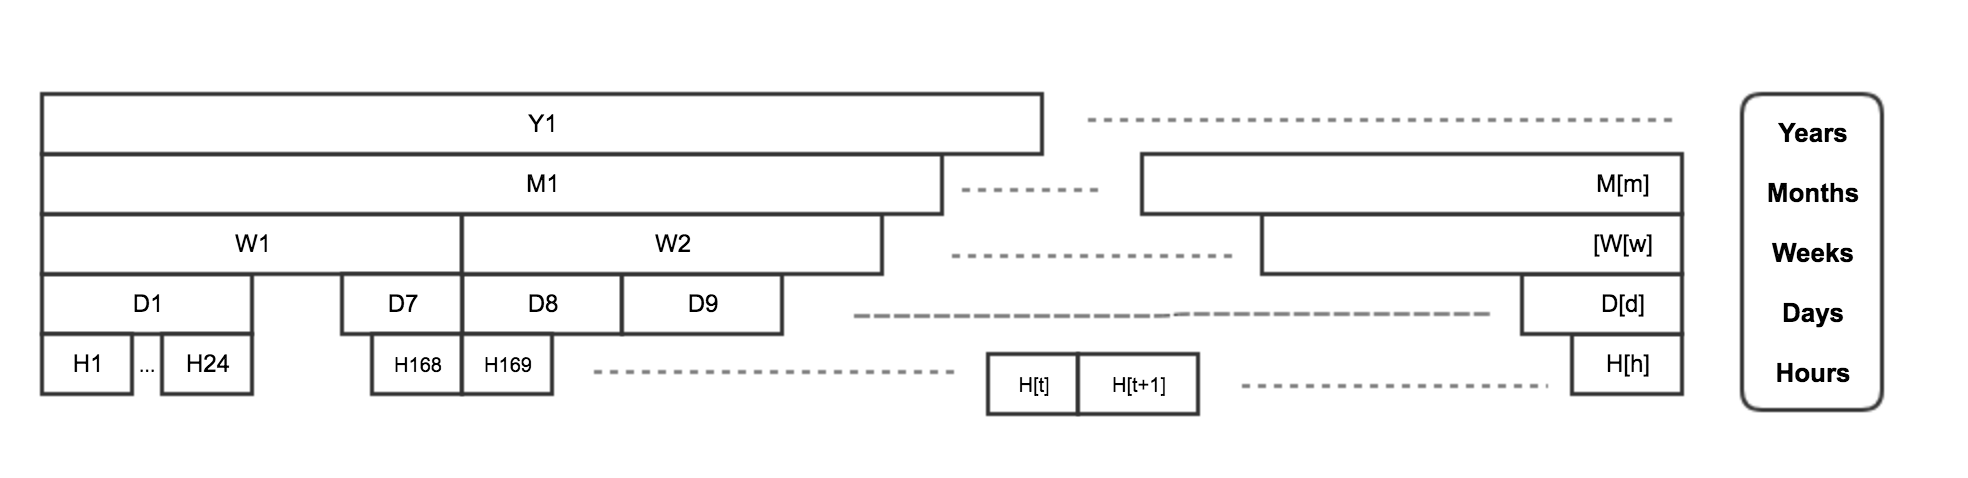
\includegraphics[width=1\linewidth]{Figs/linear-time} 

}

\caption{The time domain distributed as linear granularities}\label{fig:linear-time}
\end{figure}

\hypertarget{relationships-between-two-linear-granularities-and-association-to-periodicity}{%
\paragraph{Relationships between two linear granularities and
association to
Periodicity}\label{relationships-between-two-linear-granularities-and-association-to-periodicity}}

\citep{Bettini1998-ed} talks about the relationships of linear time
granularities and structure of a calendar and also relates them to the
notion of periodicity in time.

\begin{timedom}\label{def:finerthan}
A linear granularity G is finer than a  linear granularity H, denoted $G \preceq H$, if
for each index i, there exists an index j such that $G(i) \subset H(j)$.
\end{timedom}

\begin{timedom}\label{def:groupsinto}
A linear granularity G groups into a linear granularity H, denoted
G \trianglelefteq H 
if for each index j there exists a (possibly infinite) subset S of the integers such
that
\begin{equation}
H(j) = \bigcup_{i \in S}G(i)
\end{equation}
\end{timedom}

According to this definition, \(G \trianglelefteq H\) if each granule H
(j) is the union of some granules of G. For example,
\(Days \trianglelefteq Months\). However, this relationship is not fully
described until we associate it with periodicity. For example,
\(Days \trianglelefteq Months,\), since each month is a grouping of a
number of days, however it is also a periodical grouping. If leap year
is ignored, the periodicity of the grouping is 1 year, since each month
would be defined as the grouping of the same number of days (31, 28, or
30, depending on the month) every year. Considering leap years and all
their exceptions, the period becomes 400 years.
\textbackslash{}begin\{timedom\}\label{def:periodical} A granularity H
is periodical with respect to a granularity G if (1) G
\trianglelefteq H, and (2) there exist R,P \epsilon Z+, where R is less
than the number of granules of H, such that for all i \epsilon Z, if
H(i) = \bigcup\emph{\{j \in S\}G(j) and H (i + R) \neq \phi then H (i +
R) = \bigcup}\{j \in S\} G(j + P). \textbackslash{}end\{timedom\}

A granularity H which is periodical with respect to G is specified by:
(i) the R sets of indexes of G, \({S_0,...,S_(R-1)}\) describing the
granules of H within one period; (ii) the value of P; (iii) the indexes
of first and last granules in H, if their value is not infinite. Then,
if \({S_0,...,S_{R-1}}\) are the sets of indexes of G describing
\(H (0), . . . , H (R - 1)\), respectively, then the description of an
arbitrary granule H (j) is given by:
\(\bigcup_{i \in S_j \mod R}G(P*\lfloor j/R \rfloor + i)\).

This formula can be explained observing that H (j ) is either one of H
(0), . . . , H (R - 1) or, for the periodicity of H, is one of these
granules ``shifted'' ahead or behind on the time line of a finite number
of periods. If \(H (j ) \epsilon {H (0), . . . , H (R - 1)}\), then the
formula `j mod R' defines the index (among those in \{0,\ldots{},R -
1\}) of the granule that must be shifted to obtain H (j).The number of
periods each granule of G composing H (j mod R) should be shifted is
given by \(\lfloor j/R \rfloor\).

Granularities can be periodical with respect to other granularities,
except for a finite number of spans of time where they behave in an
anomalous way \citep{Bettini2000-vy}.

\textbackslash{}begin\{timedom\}\label{def:quasi} A granularity H is
quasi-periodical with respect to a granularity G if (1) G
\trianglelefteq H, and (2) there exist a set of intervals E1,\ldots{},Ez
(the granularity exceptions) and positive integers R,P, where R is less
than the minimum of the number of granules of H between any 2
exceptions, such that for all i \epsilon Z, if H(i) = \bigcup\emph{\{k
\in [0,k]\} G(j\_r) and H (i + R) \neq \phi and i + R \textless{}
min(E), where E is the closest existing exception after H (i)\^{}2, then
H (i + R) = \bigcup}\{k \in [0,k]\} G(j\_r + P ).
\textbackslash{}end\{timedom\}

Intuitively, the definition requires that all granules of H within the
span of time between two exceptions have the same periodical behavior,
characterized by R and P.

\begin{timedom}\label{def:BG}
**Definition: Bottom granularity** Given a granularity order relationship g-rel and a set of granularities having the same time domain, a granularity G in the set is a bottom granularity with respect to g-rel, if G g-rel H for each granularity H in the set. 
\end{timedom}

\textbf{Example:} Given the set of all granularities defined over the
time domain (Z; \textless{}), and the granularity relationship
\(\trianglelefteq\) (groups into), the granularity mapping each index
into the corresponding instant (same integer number as the index) is a
bottom granularity with respect to \(\trianglelefteq\).

\hypertarget{computation-of-linear-time-granularities}{%
\paragraph{Computation of linear time
granularities}\label{computation-of-linear-time-granularities}}

Linear time granularities are computed through an algebraic
representation for time granularities, which is referred to as calendar
algebra\citep{Ning2002-tf}. It is assumed that there exists a ``bottom''
granularity and Calendar algebra operations are designed to generate new
granularities from the bottom one or recursively, from those already
generated. Thus, the relationship between the operand(s) and the
resulting granularities are encoded in the operations.

The calendar algebra consists of two kinds of operations:
grouping-oriented and granule-oriented operations. The grouping-oriented
operations combine certain granules of a granularity together to form
the granules of the new granularity. Example can be to consider a
calendar with only two linear granularities minute and hour and hour is
generated by grouping every 60 minutes. The granule-oriented operations
do not change the granules of a granularity, but rather make choices of
which granules should remain in the new granularity. For example, one
can choose to look at the granularity ``Monday'' and hence select only
Mondays while looking at the linear granularity ``day''.

Some relevant grouping oriented operations are discussed, which will be
used in Section \ref{sec:cyclic-gran-def} to define circular and
aperiodic granularities.

\begin{itemize}
\tightlist
\item
  \textbf{The grouping operation} : Let G be a full-integer labeled
  granularity, and m a positive integer. The grouping operation
  \(Group_m(G)\) generates a new granularity G, by partitioning the
  granules of G into m-granule groups and making each group a granule of
  the resulting granularity. More precisely, \(G = Group_m(G)\) is the
  full-integer labeled granularity such that for each integer i,
  \(G(i) = \bigcup\limits_{j = (i-1)m+1}^{im} G(j)\).
\end{itemize}

\textbf{Example} :

\begin{verbatim}
- $minute = Group_{60}(second)$
- $hour = Group_{60}(minute)$,
- $day = Group_{24}(hour)$,
- $week = Group_{7}(day)$,
\end{verbatim}

where, second(1) would start a minute and likewise.

\begin{itemize}
\tightlist
\item
  \textbf{The altering-tick operation} : Let G1, G2 be full-integer
  labeled granularities, and l, k, m integers, where G2 partitions G1,
  and \(1 \leq l \leq m\). The altering-tick operation
  \(Alter^{m}_{l,k} (G2, G1)\) generates a new full-integer labeled
  granularity by periodically expanding or shrinking granules of G1 in
  terms of granules of G2. The altering-tick operation modifies the
  granules of G1 so that the lth granule of each group has
  \textbar{}k\textbar{} additional (or fewer when k \textless{} 0)
  granules of G2.
\end{itemize}

\textbf{Example} :

\begin{itemize}
\tightlist
\item
  pseudomonth =
  \(Alter^{12}_{11,-1}(day, Alter^{12}_{9,-1}(day, Alter^{12}_{6,-1}(day, Alter^{12}_{4,-1)}(day, Alter^{12}_{(2,-3)}(day, Group_{31}(day))))))\),
  where the granularity pseudomonth is generated by grouping 31 days,
  and then shrink April (4), June (6), September (9) and November (11)
  by 1 day, and shrink February (2) by 3 days. \citep{Ning2002-tf}
\end{itemize}

\hypertarget{sec:cyclic-gran-def}{%
\subsubsection{Cyclic}\label{sec:cyclic-gran-def}}

In a cyclic organization of time, the domain is composed of a set of
recurring time values. Hence, any time value can be proceeded and
succeeded by another time value (for e.g Monday comes before Wednesday
but Monday also succeeds Wednesday). Intuitively, cyclic granularities
are additional abstractions of time which are not linear and hence the
index order of linear granularities needs to be manipulated so that it
leads to repetitive categorization of time.

We propose a formalism of cyclic time granularities through the tsibble
\citep{wang2019tsibble} framework of organizing temporal data. A time
domain, as defined by Bettini, is essentially a mapping of the index set
to the time index of a tsibble. A linear granularity is a mapping of the
index set to subsets of the time domain. For example, if the time index
is days, then a linear granularity might be weeks, months or years.
Lining up with the the assumption in \citep{Bettini2000-vy} that all
linear granularities can be generated from the bottom granularity by
calendar algebraic operations, we assume that a bottom granularity
exists and is represented by the index of the tsibble.

The mappings of two linear granularities forming a cyclic granularity
can be regular or irregular. It will be regular if, for example, they
are formed by grouping operation. Grouping operation would ensure that
each granule of the resulting granularity consists of same number of
granules of bottom granularity. However, if they are formed by the
altering-tick operation, for example, granules of the resulting
granularity is composed of different number of granules of bottom
granularity. The relationship can still be periodic, depending on the
choice of periods and hence these are also useful in exploring
periodicities. However, the formalism would differ for circular (regular
mapping) and aperiodic (irregular mapping) granularities.

\hypertarget{sec:circular-gran-def}{%
\paragraph{Circular}\label{sec:circular-gran-def}}

\begin{timedom}\label{def:circular}
A circular granularity C(BG, G) relates a linear granularity G to the bottom granularity, if

\begin{equation} \label{eq:eq2}
C_{BG, G}(z) = BG(z\mod k(BG,G)) \forall z \in \mathbb{Z}^+,
BG(z) \neq \phi
\end{equation}
where,  
z denotes the index set.  
BG denotes the index of the tsibble (bottom granularity).  
G be a linear granularity, periodic with respect to BG.    
k(BG,G) be the period length of the bottom granularity with respect to linear granularity G.  
\end{timedom}

\textbf{Discussion}: Example showing circular granularities relating two
linear granularities each with bottom granularities are visually
depicted in a series of slots in the \autoref{fig:circular-gran}. Each
granule is represented by a box. The diagram also illustrates that the
granules that overlap share elements from the underlying time domain.
The first slot in the diagram shows the index set and the bottom
granularity. The index of the tsibble considered is days. G and H are
two linear granularities denoting days and weeks respectively. The
period length of days with respect to weeks is 7, hence,
\(C_{G, BG}(z)\) represented by C(BG, G) is given by \(BG(z\mod 7)\).
The circular granularity C(BG, G) consists of repetitive pattern
\{BG(0), BG(1), BG(2), BG(3), BG(4), BG(5), BG(6)\} which repeats itself
after each period length. Similarly, C(BG, H) is given by
\(BG(z\mod 14)\) since the period length of days with respect to
fortnight is 14. C(BG, H) also repeats the pattern
\({BG(0), BG(1), \dots, BG(13)}\) in every period. Hence, circular
granularities are represented as repetitive categorization of time in
the diagram.

\begin{figure}

{\centering 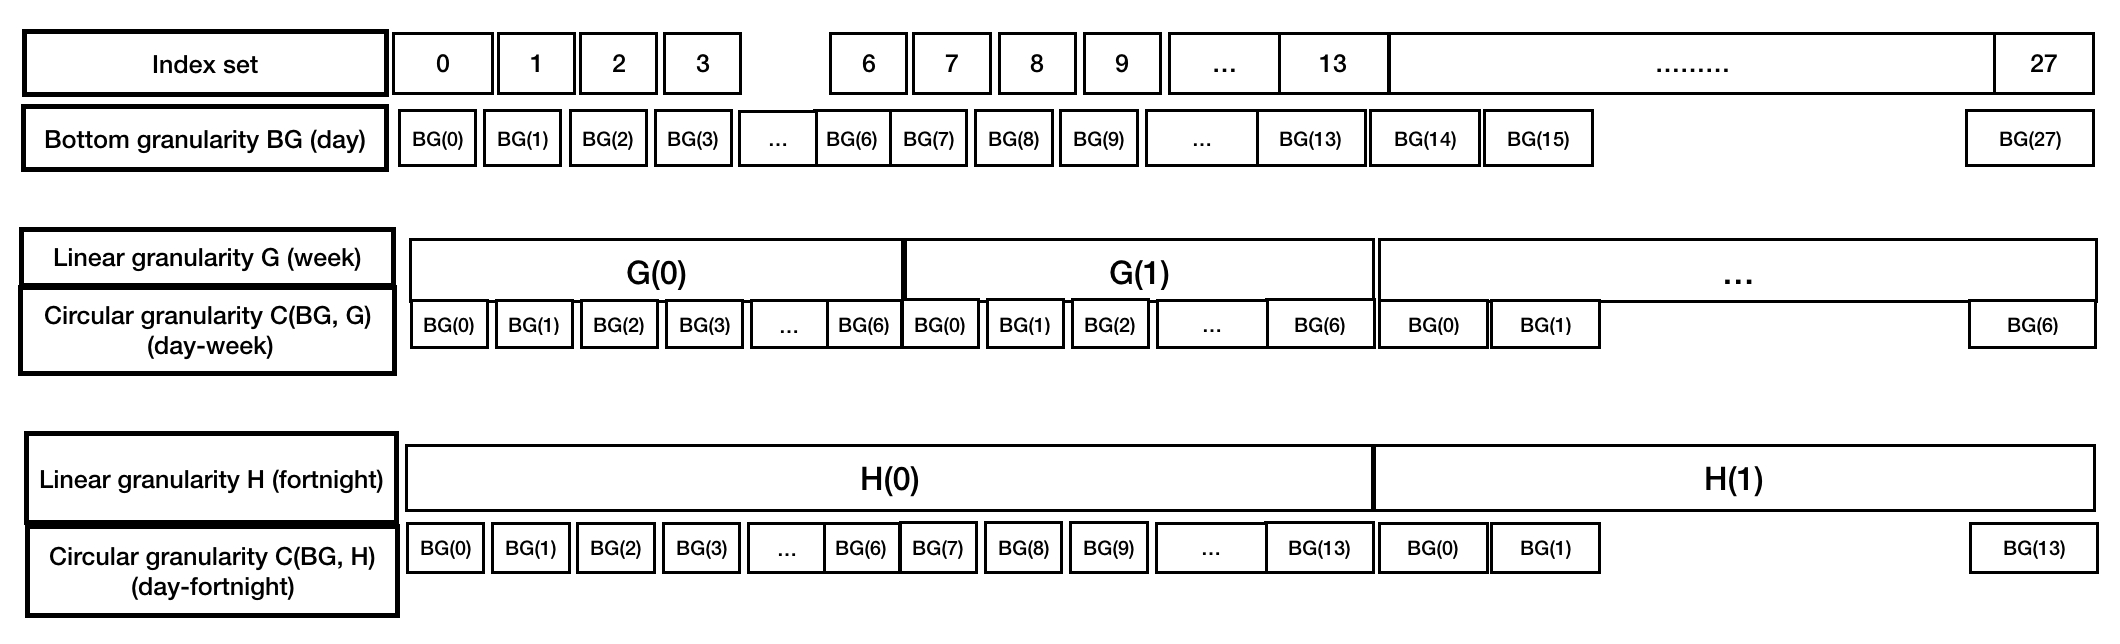
\includegraphics[width=1\linewidth]{Figs/circular-gran-diagram} 

}

\caption{Relating circular granularities and bottom linear granularity }\label{fig:circular-gran}
\end{figure}

All circular granularities can be expressed in terms of the bottom
linear granularity with equation \autoref{eq:eq2}.

In general, any circular granularity relating two linear granularity,
none of which are bottom granularity can be expressed as
\(C_{(G, H)}(z) = BG(\lfloor z/k(BG,G) \rfloor\mod k(G,H))\), where
linear granularity H is periodic with respect to linear granularity G
and k(G, H) represents the period length of G within H.

Table \ref{tab:definitions} shows representation of circular
granularities relating two linear granularities. It is possible that
none of these two linear granularities are bottom granularities. But the
representation of the resultant circular granularity will be a function
of the bottom granularity. For example, suppose the bottom granularity
is minutes, and let \(k_i\) is the period length of \(C_i\).

\begin{table}[ht]
\begin{center}
\begin{tabular}{lr@{~}lr@{~}r}
\toprule
Minute-of-Hour: & $C_1(z)$ & $= z \mod 60$ & $k_1 =$&$60$ \\
Minute-of-Day: & $C_2(z)$ & $= z \mod 60*24$ & $k_2=$&$1440$\\
Hour-of-Day: & $C_4(z)$ & $= \lfloor z/60\rfloor\mod 24$  & $k_3 =$&$24$ \\
Hour-of-Week: & $C_6(z)$ & $= \lfloor z/60\rfloor\mod 24*7$  & $k_4=$&$168$\\
Day-of-Week: & $C_7(z)$ & $= \lfloor z/24*60\rfloor \mod 7$ & $k_5=$&$7$\\
\bottomrule
\end{tabular}
\end{center}
\caption{Illustrative circular granularities with time index in minutes}
\label{tab:definitions}
\end{table}

\hypertarget{sec:aperiodic-gran-def}{%
\subsubsection{Aperiodic}\label{sec:aperiodic-gran-def}}

An \textbf{Aperiodic granularity} can not be defined using modular
arithmetic. The modulus for these type of calendar categorizations are
not constant due to irregular mapping with bottom granularities. For
example,\autoref{tab:aperiodic} shows some example of aperiodic
granularities (\(A_i\)) and plausible choices of period
lengths(\(k_i\)). The coarse granularity is assumed as the period within
which the finer granularity will repeat its behavior aperiodically.

\begin{table}[ht]
\begin{center}
\begin{tabular}{lr@{~}lr@{~}r}
\toprule

Day-of-Month: & $A_1(z)$ &  $k_1=31, 30, 29, 28$\\
Hour-of-Month: & $A_2(z)$ & $k_2=24*31, 24*30, 24*29, 24*28$\\
Day-of-Year: & $A_3(z)$ & $k_3=366, 365$\\
Week-of-Month: & $A_4(z)$ & $k_4=5, 4$\\ 
\bottomrule
\end{tabular}
\end{center}
\caption{Illustrative aperiodic circular granularities with potential period lengths}
\label{tab:aperiodic}
\end{table}

\textbf{Definition: Aperiodic granularity} An aperiodic granularity
A(AG, BG) that relates linear granularities AG and bottom granularity
BG, with AG being periodical with respect to BG, is given by

\begin{equation}\label{eq:eq3}
A_{BG, AG}(z) = BG(z - \sum_{w=0}^{k-1}\vert T_{w \mod R'} \vert), z \in T_k
\end{equation} where,\\
z denotes the index set (index of BG), R' denotes the number of granules
of AG in each period of BG,\\
\(T_w\) are the sets of indices of BG describing \(AG(w)\) such that
\(AG(w) = \bigcup_{z \in T_w}BG(z)\), and \(T_w = 0\) for
\(w \epsilon Z_{<0}\)\\
\(\vert T_w \vert\) is the cardinality of set \(T_w\).

Since AG is periodical with respect to BG, from definition of ``Groups
periodically into'' the following holds true:

\begin{itemize}
\tightlist
\item
  \(BG \trianglelefteq AG\)
\item
  \(AG(w) = \bigcup_{z \in T_w \mod R}BG(P'*\lfloor w/R' \rfloor + z)\),
  where P' denotes the period of the granularity BG.
\end{itemize}

\textbf{Discussion}: Example showing aperiodic granularities relating
two linear granularities each with bottom granularities are visually
depicted in a series of slots in \autoref{fig:aperiodic-gran}. Each
granule is represented by a box. Similar to \autoref{fig:circular-gran},
the granules that overlap share elements from the underlying time domain
and the first slot shows the index set and the bottom granularity. Two
linear granularities AG and AH are considered, where
\(AG = Alter^{2}_{(1,-1)}(BG, Group_3(BG))\) and
\(AH = Alter^{2}_{(1,-2)}(BG, Group_7(BG))\). This implies that AG is
made up by shrinking every 1st granule of Group\_3(BG) by 1 granule and
AH is made up of shrinking every 1st granule of Group\_3(BG) by 2
granules. Number of granules of AG and AH in each period of BG is 2, but
the number of granules of BG in each of those granules are different.
A(BG, AG) and A(BG, AH) are repetitive categorization of time, similar
to circular granularities, except that the number of granules of BG is
not necessarily the same across different granules of AG or AH. For AG,
R' = 2, P'= 5, \(T_0\) = \{0,1\} and \(T_1\) = \{2, 3, 4\}. For AH, R' =
2, P'= 12, \(T_0\) = \{0, 1, 2, 3, 4, 5, 6\} and \(T_1\) = \{7, 8, 9,
10, 11\}, then we will have \autoref{eq:eq4} and \autoref{eq:eq5}.

\begin{equation} \label{eq:eq4}
\begin{split}
A(BG,AG)(8) & = BG(8 - \sum_{w=0}^{3-1}\vert T_{w \mod 2}\vert) , 8 \in T_{3} \\
  & = BG(8 - \sum_{w=0}^{2}\vert T_{w\mod 2}\vert) \\
  & = BG(8 - \sum_{w=0}^{2}\vert T_{w\mod 2}\vert) \\
  & = BG(8 - \vert T_{0 \mod 2}\vert - \vert T_{1 \mod 2}\vert - \vert T_{2 \mod 2}\vert) \\
  & = BG(8 - 2*\vert T_{0 \mod 2}\vert - \vert T_{1 \mod 2}\vert) \\
  & = BG(8 - 2*2 - 3) \\
  & = BG(1) \\
\end{split}
\end{equation}

\begin{equation} \label{eq:eq5}
\begin{split}
A(BG,AH)(10) & = BG(10 - \sum_{w=0}^{1-1}\vert T_{w \mod 2}\vert) ,  10 \in T_{1}  \\
  & = BG(10 - \sum_{w=0}^{0}\vert T_{w\mod 2}\vert) \\
  & = BG(10 - \vert T_{0 \mod 2}\vert) \\
  & = BG(10 - \vert T_{0}\vert) \\
  & = BG(10 - 7) \\
  & = BG(3) \\
\end{split}
\end{equation}

\begin{figure}

{\centering 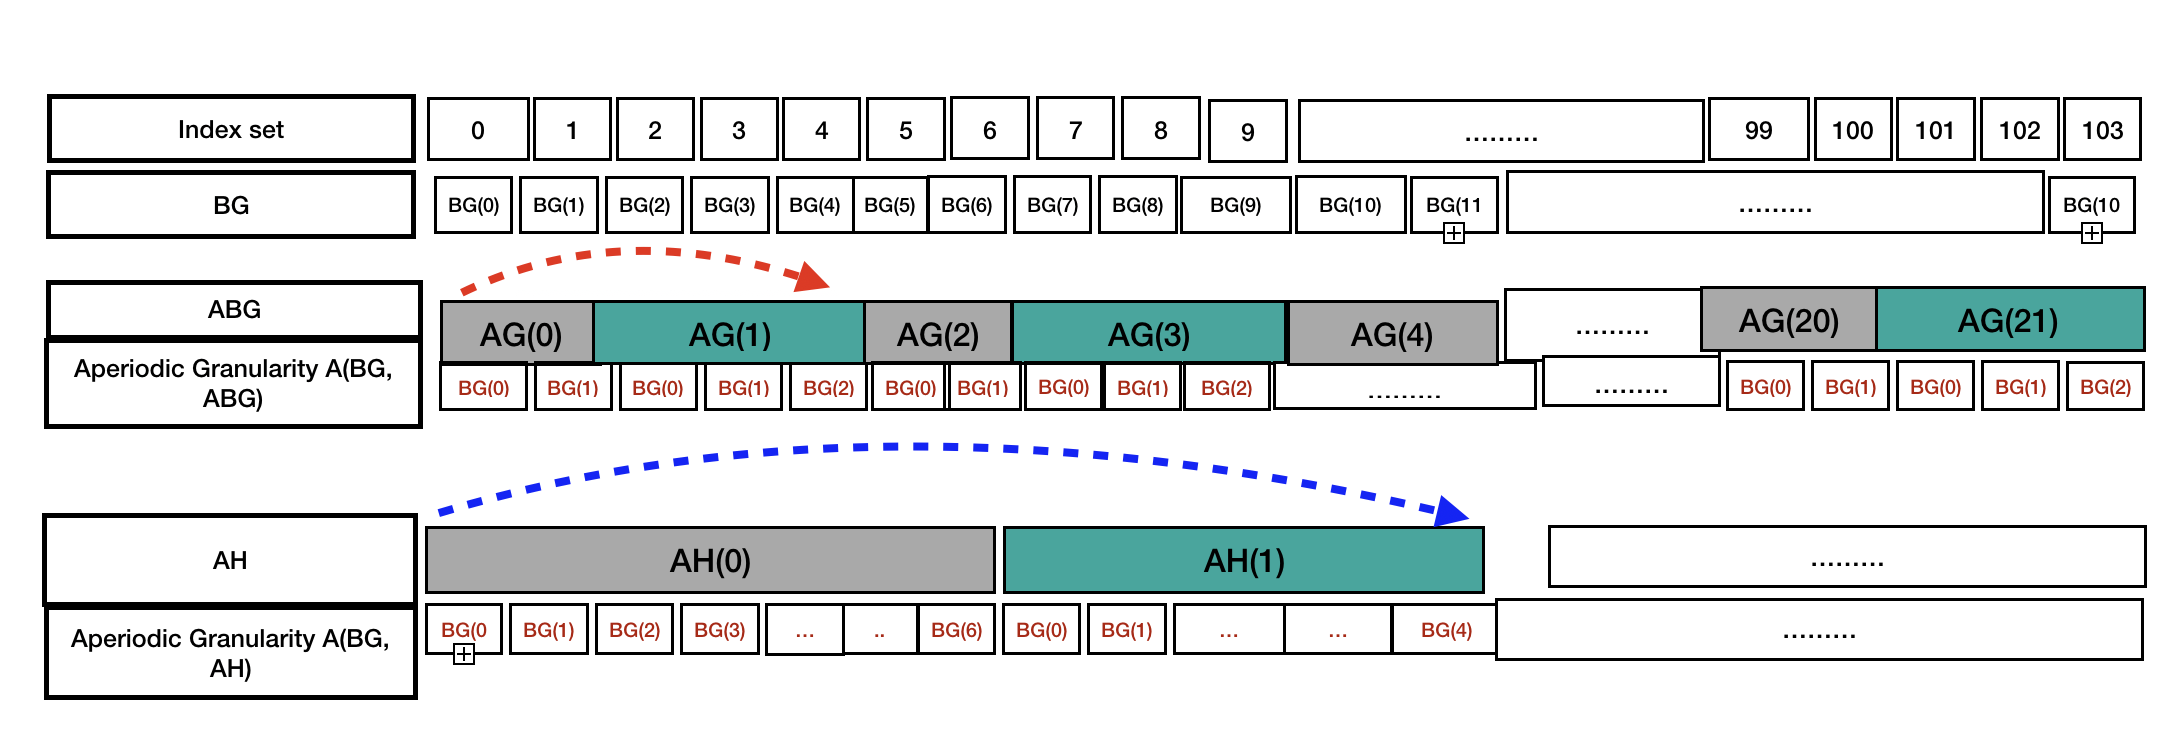
\includegraphics[width=1\linewidth]{Figs/aperiodic-granv1} 

}

\caption{Relating circular granularities and bottom linear granularity }\label{fig:aperiodic-gran}
\end{figure}

If we ignore leap years and all its exception, the periodicity of the
grouping (days, months), P' = 365, R' = 12, since each month would be
defined as the grouping of the same number of days (31, 28, or 30,
depending on the month) every year. Considering leap years and all their
exceptions, period is 400 years and hence \(P' = (3*365 + 366)\),
\(R' = 12*400\). \autoref{eq:eq3} can be useful to find the aperiodic
granularity day-of-month in both of these cases, since the grouping is
periodic is both cases.

The linear granularities G, H, AG and AH considered in the definitions
of circular and aperiodic granularities are all periodic with respect to
the bottom granularity. The only difference is G, H have regular
mapping, whereas, G1 and G2 have irregular mapping with respect to BG.
It can be noted here that if a linear granularity AG is quasi-periodic
with respect to BG, then \autoref{eq:eq3} can be modified as follows to
account for exceptions \(E = [e_{begin}, e_{end}]\) (by Definition
\autoref{def:quasi})

\begin{equation}\label{eq6}
A_{BG, AG}(z) = BG(z - \sum_{w=0}^{k-1}\vert T_{w} \vert - \sum_{u=0}^{e_k}\vert E_{u} \vert)
\end{equation}

for \(z \in T_k\) and \(e_k\) is the number of exceptions in
\(\bigcup\limits_{w = 0}^{k} T_w\) and
\(E_{u} = [e_{begin}(u), e_{end}(u)]\).

\hypertarget{sec:order}{%
\subsection{Order: Single vs.~Multiple}\label{sec:order}}

The hierarchical structure of time creates a natural nested ordering
which can produce \textbf{single-order-up} or \textbf{multiple-order-up}
granularities. We shall use the notion of a hierarchy table and order to
define them.

\textbf{Definition: Order} of a linear granularity can be comprehended
as the level of graininess associated with a linear granularity. If we
consider two linear granularities G and H, such that G is finer than or
groups into H (by Definitions \ref{def:finerthan},
\ref{def:groupsinto}), then H is of higher order than G.

\textbf{Notation: Hierarchy table} Let \(H_n: (G, C, k)\) be a hierarchy
model containing n linear granularities. \(G_{l}\) represents the linear
granularity of order l and \(k(l,m)\) represents the period length of
\(G_{l}\) with respect to \(G_{m}\) and \(C_{G(l),G(m)}\) represents the
circular granularity that relates linear granularity of order l and m,
\(\forall l,m \in n, l<m\).

In a hierarchy table, linear granularities are arranged from lowest to
highest order of linear granularities.

We refer to granularities which are nested within multiple levels as
\textbf{multiple-order-up} granularities and those concerning a single
level as \textbf{single-order-up} granularities. Let us look at few
calendars to see examples of single and multiple order-up granularities.

\hypertarget{sec:multiplefromsingle}{%
\subsubsection{Computation of multiple-order from
single-order}\label{sec:multiplefromsingle}}

\begin{equation} \label{eq7}
\begin{split}
C_{(G_l,G_m)}(z) & = C_{G_l,G_{l+1}}(z) + k(l, l+1)(C_{(G_(l+1),G_m)}(z)-1) \\  
  & =   C_{(G_l,G_{l+1}}(z) + k(l, l+1)[ C_{G_{l+1},G_{l+2}}(z) + k(l+1, l+2)( C_{G_{l+2}, G_m}(z) - 1) - 1] \\
  & =  C_{(G_l,G_{l+1}}(z) + k(l, l+1)(C_{G_{l+1},G_{l+2}}(z) - 1) + k(l, l+1)k(l+1, l+2)(C_{G_{l+2}, G_{m}} - 1)\\
  & =  C_{(G_l,G_{l+1}}(z) + k(l, l+1)(C_{G_{l+1},G_{l+2}}(z) - 1) + k(l, l+2)(C_{G_{l+2},G_{l+m}}(z) - 1)\\
  &\vdots\\
  & = \sum_{i=0}^{m - l - 1} k(l, l+i)(C_{G_{l+i},G_{l+i+1}}(z) - 1)\\
\end{split}
\end{equation}

\textbf{Example:} So far we have used the Gregorian calendar as it is
the most widely used calendar. But it is far from being the only one.
All calendars fall under three types - solar, lunar or
lunisolar/solilunar but the day is the basic unit of time underlying all
calendars. Various calendars, however, use different conventions to
structure days into larger units: weeks, months, years and cycle of
years. The French revolutionary calendar divided each day into 10
``hours'', each ``hour'' into 100 ``minutes'' and each ``minute'' into
100 ``seconds''. Nevertheless, for any calendar a hierarchy can be
defined. For example, in Mayan calendar, one day was referred to as 1
kin and the calendar was structured as follows \citep{Reingold2001-kf}:

\begin{itemize}
\tightlist
\item
  1 kin = 1 day
\item
  1 uinal = 20 kin
\item
  1 tun = 18 uinal
\item
  1 katun = 20 tun
\item
  1 baktun = 20 katun
\end{itemize}

Thus, the hierarchy table for the Mayan calendar would look like the
following:

\begin{longtable}[]{@{}lll@{}}
\toprule
G & C & k\tabularnewline
\midrule
\endhead
kin & kin-of-uinal & 20\tabularnewline
uinal & uinal-of-tun & 18\tabularnewline
tun & tun-of-katun & 20\tabularnewline
katun & katun-of-baktun & 20\tabularnewline
baktun & 1 & 1\tabularnewline
\bottomrule
\end{longtable}

Examples of multiple-order-up granularities can be kin-of-tun or
kin-of-baktun whereas examples of single-order-up granularities may
include kin-of-uinal, uinal-of-tun etc.

Let us use the equation \ref{eq:eq3} to compute the multiple-order-up
granularity uinal\_katun for Mayan calendar, which is periodic and
regular.

\begin{equation} \label{eq8}
\begin{split}
C(uinal, baktun) & = C(uinal, tun) + kuinal, tun)C(tun,katun) + C(uinal, katun)C(katun, baktun) \\
              & = \lfloor z/20\rfloor \mod 18  + 20*\lfloor z/20*18\rfloor \mod 20 + 20*18*20\lfloor z/20*18*20\rfloor \mod 20 \\
\end{split}
\end{equation}

\hypertarget{sec:singlefrommultiple}{%
\subsubsection{Computation of single-order from
multiple-order}\label{sec:singlefrommultiple}}

For a hierarchy table \(H_n: (G, C, k)\) with
\(l_1, l_2, m_1, m_2 \in {1, 2, \dots, n}\) and \(l_2<l_1\) and
\(m_2>m_1\), we have

\begin{equation} \label{eq9}
C_{G_{l1}, G_{m1}}(z) = C_{G_{l2}, G_{m2}}(\lfloor z/k(l_2,l_1) \rfloor\mod k(m_1, m_2))
\end{equation}

\textbf{Example:} Considering the same example of Mayan Calendar, it is
possible to compute the single-order-up granularity tun-of-katun given
the multiple-order-up granularity uinal-baktun using equation
\ref{eq:eq5}

\begin{equation} \label{eq10}
\begin{split}
C(tun, katun) =  \lfloor C(uinal, baktun)(z)/18\rfloor \mod 20 \\
\end{split}
\end{equation}

In \autoref{sec:singlefrommultiple} and
\autoref{sec:multiplefromsingle}, we assume that all single order
granularities are circular.What happens when we have a mix of circular
and aperiodic granularities.

Let us turn to Gregorian calendar for addressing this case. Suppose we
have a hierarchy table using some linear granularties from Gregorian
calendar. Since months consists of unequal number of days, any temporal
unit which is higher in order than months will also have unequal number
of days. This is an example of a hierarchy structure which has both
circular and aperiodic single-order-up granularities. The
single-order-up granularity day\_month is aperiodic. Any single-order-up
granularities which are formed by units below days are periodic.
Similarly, all single-order-up granularities which are formed using
units whose orders are higher than months are also periodic.

\begin{longtable}[]{@{}lll@{}}
\toprule
G & C/A & k\tabularnewline
\midrule
\endhead
minute & minute-of-hour & 60\tabularnewline
hour & hour-of-day & 24\tabularnewline
day & day-of-month & ``aperiodic''\tabularnewline
month & month-of-year & 12\tabularnewline
year & 1 & 1\tabularnewline
\bottomrule
\end{longtable}

There can be three scenarios for obtaining multiple-order-granularities
here: - granularities relating two linear granularities whose orders are
less than day - granularities relating two linear granularities whose
orders are more than month - granularities relating two linear
granularities with order at most day and another with order at least
month

The single order-up granularites resulting from the first two cases are
periodic and has been handled in \autoref{sec:singlefrommultiple} and
\autoref{sec:multiplefromsingle}. The calendar categorization resulting
from the last case are aperiodic. Examples might include day of the
quarter or hour of the month. Let us consider the computation of
\(A_{hour, month}\) given single order-up granularities
\(A_{hour, day} = 12\), \(A_{day, month} = 20\) and
\(C_{month, year} = 9\).

\begin{equation} \label{eq11}
\begin{split}
A_{(hour, month)} & = (\sum_{w=0}^{9 - 1}(\vert T(w)\vert) +  20)/24 + 12 \\
                  & = (\sum_{w=0}^{C_{month, year} - 1}(\vert T(w)\vert) +  A_{day, month})*k(hour_day) + A_{hour, day} \\
                  & = (A{day_year} - 1)*k(hour_day) + A_{hour, day} \\
\end{split}
\end{equation} where, \(month(w) = \bigcup_{z \in T_w}day(z)\)

Clearly, the computation of multiple order-up granularities become more
involved with aperiodic mappings of linear granularities in the calendar
structure. With one aperiodic granularity, we can write the following:

A\_\{P, Q)\} \& = (A\{AG\_Q\} - 1)*k(P\_AG) + A\_\{P, AG\} \{TO REVISE:
many aperiodic granularties not to be included\}

\hypertarget{sec:synergy}{%
\section{Synergy of cyclic time granularities}\label{sec:synergy}}

Before exploring the behavior of a ``dependent variable'' across time
granularities, it is important to know how these granularities interact
with each other. If two time granulaties of interest interact, the
relationship between each of the interacting variables and the dependent
variable will depend on the value of the other interacting variable. To
define a general framework, we define harmony and clashes.

\hypertarget{harmony-and-clashes}{%
\subsection{Harmony and Clashes}\label{harmony-and-clashes}}

Suppose we have two cyclic granularities \(C_1\) and \(C_2\), such that
\(C_1\) maps index set to a set \(\{A_1,A_2,A_3,\dots, A_n\)\}, and
\(C_2\) maps index set to a set \(\{B_1,B_2,B_3,\dots, B_m\)\}. That is,
let \(S_{ij}\) be the set of index set such that for all
\(s \in S_{ij}\), \(C_1(s) = i\) and \(C_2(s) = j\). Since, \(C_1\) has
n levels and \(C_2\) has m levels there will be \(nm\) such sets
\(S_{ij}\).Now, many situations can lead to any of these sets being
empty. Let us discuss the following cases, where one or more of these
sets can be empty.

Firstly, empty combinations can arise due to the structure of the
calendar or hierarchy. These are called ``structurally'' empty
combinations. Let us take a specific example, where \(C_1\) maps row
numbers to Day-of-Month and \(C_2\) maps row numbers to Week-of-Month.
Here \(C_1\) can take 31 values while \(C_2\) can take 5 values. There
will be \(31\times 5=155\) sets \(S_{ij}\) corresponding to the possible
combinations of WOM and DOM. Many of these are empty. For example
\(S_{1,5}\), \(S_{21,2}\), etc.This is also intuitive since the first
day of the month can never correspond to fifth week of the month. These
are structurally empty sets in that it is impossible for them to have
any observations.

Secondly, empty combinations can turn up due to differences in event
location or duration in a calendar. These are called ``event-driven''
empty combinations. Again, let us consider a specific example to
illustrate this. Let \(C_1\) be DOW and \(C_2\) be
WorkingDay/NonWorkingDay. Here \(C_1\) can take 7 values while \(C_2\)
can take 2 values. So there are 14 sets \(S_{ij}\) corresponding to the
possible combinations of DOW and WD/NWD. While potentially all of these
can be non-empty (it is possible to have a public holiday on any DOW),
in practice many of these combinations will probably have very few
observations. For example, there are few if any public holidays on
Wednesdays or Thursdays in any given year in Melbourne.

Thirdly, empty combinations can be a result of how granularities are
constructed. Let \(C_1\) maps row numbers to ``Business days'', which
are days from Monday to Friday except holidays and \(C_2\) is
Day-of-Month. Then the weekends in Days-of-Month would not correspond to
any Business days and would have missing observations due to the way the
granularities are constructed. This is different from the structurally
empty combinations because structure of the calendar does not lead to
these missing combinations, but the construction of the granularity
does. Hence, they are referred to as ``build-based'' empty combinations.

An example when there will be no empty combinations could be where
\(C_1\) maps row numbers to Day-of-Week and \(C_2\) maps row numbers to
Month-of-Year. Here \(C_1\) can take 7 values while \(C_2\) can take 12
values. So there are \(12\times7=84\) sets \(S_{ij}\) corresponding to
the possible combinations of DOW and MOY. All of these are non-empty
because every DOW can occur in every month.

Therefore, pair of circular/aperiodic granularities which lead to
structurally, event-driven or build-based empty-combinations are
referred to as to as \textbf{clashes}. And the ones that do not lead to
any missing combinations are called \textbf{harmonies}.

\hypertarget{sec:visualization}{%
\section{Visualization}\label{sec:visualization}}

Creating a visualisation requires a number of nuanced judgements. We
exploit some features of layers and faceting \citep{Wilkinson1999-nk}
and \citep{Wickham2009-pk} to come up with a recommendation system while
visualizing the distribution of the ``dependent'' variable across
bivariate temporal granularities. The general framework of visualizing
the distribution invloves a faceting approach with one temporal
granularity plotted along the x-axis, the other one across facet and the
dependent time series variable on the y-axis. Different distribution
plots might be appropriate depending on which features of the
distrbution we are interested to look at, the levels of time
granularities being plotted, how granularities interact and number of
observations available. We will look at each of these aspects separately
and analyze the effect of each on visualization.

While we accomplish that, we need to bear in mind that any customized
species of visualization might be constructed by varying the set of
mappings between data properties and visual attributes such as position,
shape and color. We are trying to address problems where even with good
aesthetic qualities and good data, the graph might be confusing or
misleading because of how people process the information.

\hypertarget{choice-of-plots}{%
\subsection{Choice of Plots}\label{choice-of-plots}}

There are several ways to plot statistical distributions. The displayed
probabilities in these plots are either computed using kernel density
estimation methods or empirical statistical methods. The latter do not
allow us to see the shape, skewness, nature of the tail or
multi-modality with so much clarity as the former. However, they avoid
much clutter, where some specific probabilities representing typical and
extreme behavior are on focus. The probabilities displayed are based on
actual data, which is aligned to principles that governed Tukey's
original boxplot. Density plots which uses a kernel density estimate to
show the probability density function of the variable can show the
entire distribution, unlike discretizing the distribution and showing
only parts of it. They can be useful in spotting multimodality, however,
they might become obscuring with too many categories and information on
the entire distribution can add to cognitive load. Also, the
probabilities in density plot are estimated through kernel density
estimation and thus makes assumptions when selecting kernel or
bandwidth. As a result, the plot shows smooth summaries based on the
assumptions and not only on actual observations. The density based
visualizations are subject to the same sample size restrictions and
challenges that apply to any density estimation. In practice, the
densities are estimated reasonably with at least 30 observations. Even
with sample sizes of several hundred, however, choosing too large a
value for bandwidth can cause the estimate to oversmooth the data.

We will discuss few conventional and recent ways to plot distributions
using both of these methods.

\hypertarget{empirical-methods}{%
\subsubsection{Empirical methods}\label{empirical-methods}}

Most commonly used techniques to display a distribution of data include
the histogram (Karl Pearson), which shows the prevalence of values
grouped into bins and the box-and-whisker plots \citep{Tukey1977-jx}
which convey statistical features such as the median, quartile
boundaries, hinges, whiskers and extreme outliers. The box plot is a
compact distributional summary, displaying less detail than a histogram.
Due to wide spread popularity and simplicity in implementation, a number
of variations are proposed to the original one which provides alternate
definitions of quantiles, whiskers, fences and outliers. Notched box
plots \citep[1978]{Mcgill1978-hg} has box widths proportional to the
number of points in the group and display confidence interval around
medians aims to overcome some drawbacks of box plots. The standard box
plot and all of these variations are helpful to get an idea of the
distribution at a glance. Moreover, for data less than 1000
observations, detailed estimates of tail behavior beyond the quartiles
are not trustworthy. Also, the number of outliers is large for larger
data set since number of outliers is proportional to the number of
observations.

The letter-value box plot \citep[2006]{Hofmann2017-sg} was designed to
adjust for number of outliers proportional to the data size and display
more reliable estimates of tail. ``outliers'' in letter value plots are
those observations beyond the most extreme letter value. The letter
values are shown till the depths where the letter values are reliable
estimates of their corresponding quantiles and hence might lead to a lot
of letter values being shown and leading to overload of information in
one plot.

Quantile plots visually portray the quantiles of the distribution of
sample data. Much like the quartiles divide the data set equally into
four equal parts, extensions include dividing the data set even further.
These plots are referred to as ``quantile'' plots. For example, number
of quantiles would be 9 for a decile plot and 99 for percentile plot. It
avoids much clutter and just enable us to focus on specific
probabilities, typically representing typical and extreme behaviors. A
large data set is required for the extreme percentiles to be estimated
with any accuracy. These plots can display any quantiles instead of
quartiles in a traditional boxplot. When reviewing a boxplot, an outlier
is defined as a data point that is located outside the fences
(``whiskers'') of the boxplot (e.g: outside 1.5 times the interquartile
range above the upper quartile and below the lower quartile). However,
outliers are open to interpretation and not shown in an quantile plot.

\hypertarget{kernel-density-estimation-methods}{%
\subsubsection{Kernel density estimation
methods}\label{kernel-density-estimation-methods}}

Traditional ways to visualize densities include violin plots
\citep[1998]{Hintze1998-zi}. The shape of the violin represents the
density estimate of the variable. The more data points in a specific
range, the larger the violin is for that range. Adding two density plots
gives a symmetric plot which makes it easier to see the magnitude of the
density and compare across categories, enabling easier detection of
clusters or bumps within a distribution.

The summary plot \citep[2010]{Potter2010-qc} combines a minimal box plot
with glyphs representing the first five moments (mean, standard
deviation, skewness, kurtosis and tailings), and a sectioned density
plot crossed with a violin plot (both color and width are mapped to
estimated density), and an overlay of a reference distribution. This
suffers from the same problem as boxplots or violin plot, as it is
combination of those two.

A Ridge line plot (sometimes called Joy plot) shows the distribution of
a numeric value for several groups. Distribution can be represented
using histograms or density plots, all aligned to the same horizontal
scale and presented with a slight overlap. A clear advantage over
boxplots is that these plots allow us to see multimodality in the
distribution. However, these plots can be obscuring when there is
overlap of distribution for two or more categories of the y-axis. Also,
if there are lot of categories, it is difficult to compare the height of
the densities across categories.

The highest density region (HDR) box plot proposed by
\citep{Hyndman1996-ft} displays a probability density region that
contains points of relatively highest density. The probabilities for
which the summarization is required can be chosen based on the
requirement. These regions do not need to be contiguous and help
identify multi-modality.

Given a context, it is good to be conversant with the benefits and
challenges while choosing a distribution plot. As a general rule, if we
have too many categories, the quantile plots are useful for comparing
patterns, whereas, other more involved methods of plotting are useful
for studying anomalies, outlier or multimodal behavior.

\hypertarget{effect-of-levels-of-temporal-granularities}{%
\subsubsection{Effect of levels of temporal
granularities}\label{effect-of-levels-of-temporal-granularities}}

The levels of the two granularities plotted have an impact on the choice
of plots since space and resolution might become a problem if the number
of levels are too high. The criteria for different levels could be based
on usual cognitive power while comparing across facets and display size
available to us. Plot choices will also vary depending on which
granularity is placed on the x-axis and which one across facets.

Levels are categorized as very high/high/medium/low each for the facet
variable and the x-axis variable. Default values for these levels are
chosen based on levels of common temporal granularities like day of the
month, day of a fortnight or day of a week. Any levels above 31 can be
considered as very high, any levels between 14 to 31 can be taken as
high and that between 7 to 14 can be taken as medium and below 7 as low.
31, 14 and 7 are the levels of days-of-month, days-of-fortnight and
days-of week respectively.

The following principles are useful while choosing distribution plots
given two temporal granularities.

\begin{itemize}
\item
  If levels of both granularity plotted are low/medium, then any
  distribution plots might be chosen depending on which feature of the
  distribution needs focus.
\item
  If level of the granularity plotted across x-axis is more than medium,
  ridge plots should be avoided to escape overlap of categories.
\item
  If level of the granularity plotted across x-axis is more than or
  equal to high, quantile plots are preferred.
\item
  If levels of any granularity plotted are more than medium, empirical
  based methods of distribution visualizing are preferred as they use
  less space by design than most density based methods.
\end{itemize}

\hypertarget{effect-of-synergy-of-time-granularities}{%
\subsection{Effect of synergy of time
granularities}\label{effect-of-synergy-of-time-granularities}}

In Section \ref{sec:synergy}, we discussed how pairs of granularities
can have empty combinations either due to structure of calendar, event
location or duration or due to the way they are built. In this section,
we will see how these empty combinations affect the visualization when a
dependent variable is plotted against these granularities.

For illustration, distribution of half-hourly electricity consumption of
Victoria is plotted across different time granularities in each of the
panel in \autoref{fig:allFig}. \autoref{fig:allFig} (a) shows the letter
value plot across days of the month faceted by months like January,
March and December. \autoref{fig:allFig} (c) shows box plot across days
of the year by the 1st, 15th, 29th and 31st days of the month.
\autoref{fig:allFig} (d) showing violin plot across days of the month
faceted by week of the month. \autoref{fig:allFig} (e), variations
across week of the year conditional on week of the month can be observed
through a ridge plot and \autoref{fig:allFig} (f) shows decile plots
across day of the year and month of the year.

Clearly, in \autoref{fig:allFig}, we observe that some choices of time
granularities work and others do not. In \autoref{fig:allFig} (c), there
will be no observations for some combinations ``Day-of-Month'' and
``Day-of-Year''. In particular, the 1st day of the month can never
correspond to 2nd, 3rd or 4th day of the year. On the contrary, for
\autoref{fig:allFig} (a), we will not have any combinations with zero
combinations because every ``Day-of-Week'' can occur in any
``Month-of-Year''. Thus the graphs that don't work are those where many
of the combination sets are empty. In other words, if there are levels
of time granularities plotted across x-axis which are not spanned by
levels of the time granularities plotted across facets or vice versa, we
will have empty sets leading to potential ineffective graphs. We
hypothesize that the synergy of these granularities are in play while
deciding if the resulting plot would be a good candidate for exploratory
analysis.

We redefine harmony and clashes as follows: harmonies are pairs of
granularities that aid exploratory data analysis, and clashes are pairs
that are incompatible with each other for exploratory analysis. As a
result, we should avoid plotting clashes as they hinder the exploratory
process by having missing combinations of time granularities in each
panel.

\begin{figure}

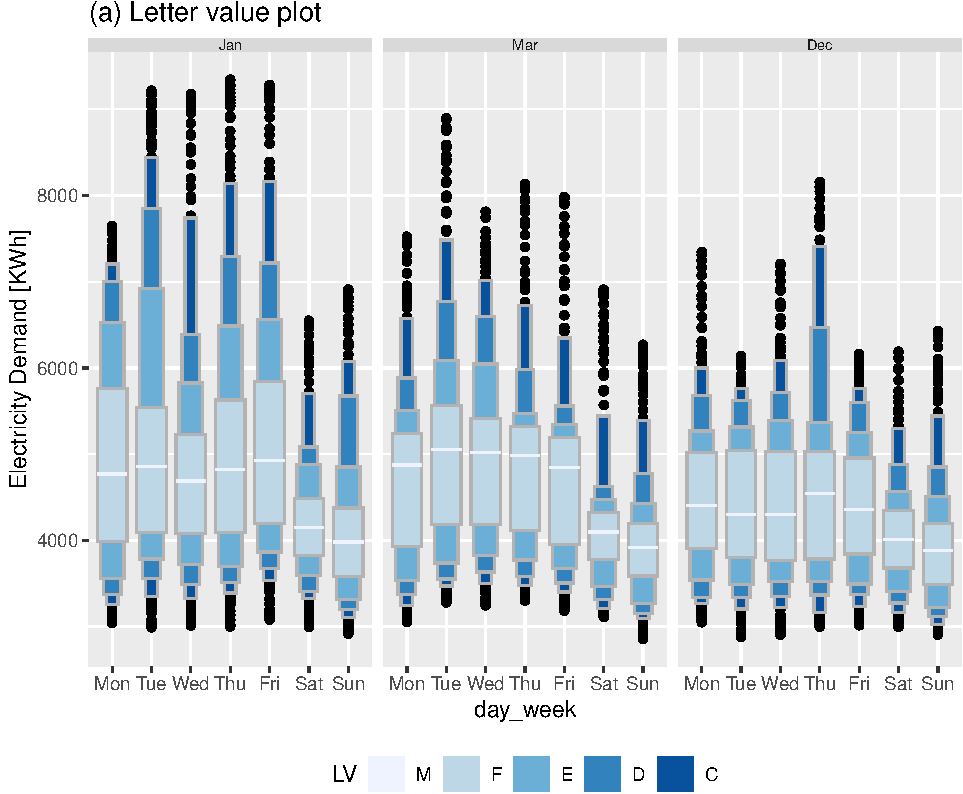
\includegraphics[width=0.5\linewidth]{figure/allFig-1} 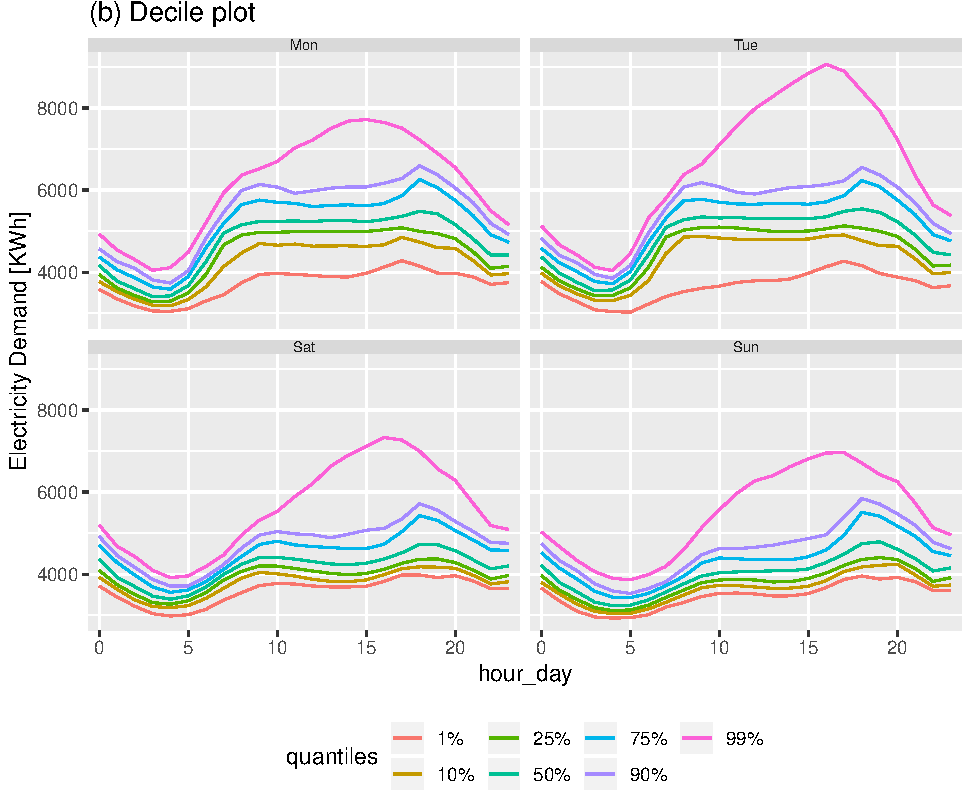
\includegraphics[width=0.5\linewidth]{figure/allFig-2} 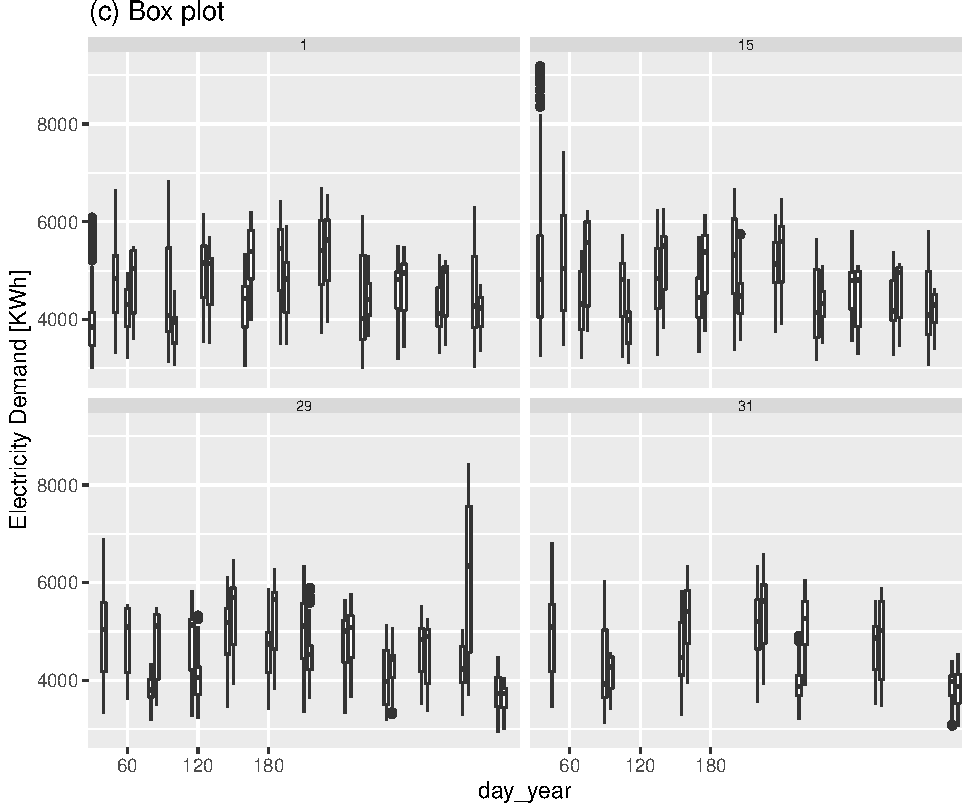
\includegraphics[width=0.5\linewidth]{figure/allFig-3} 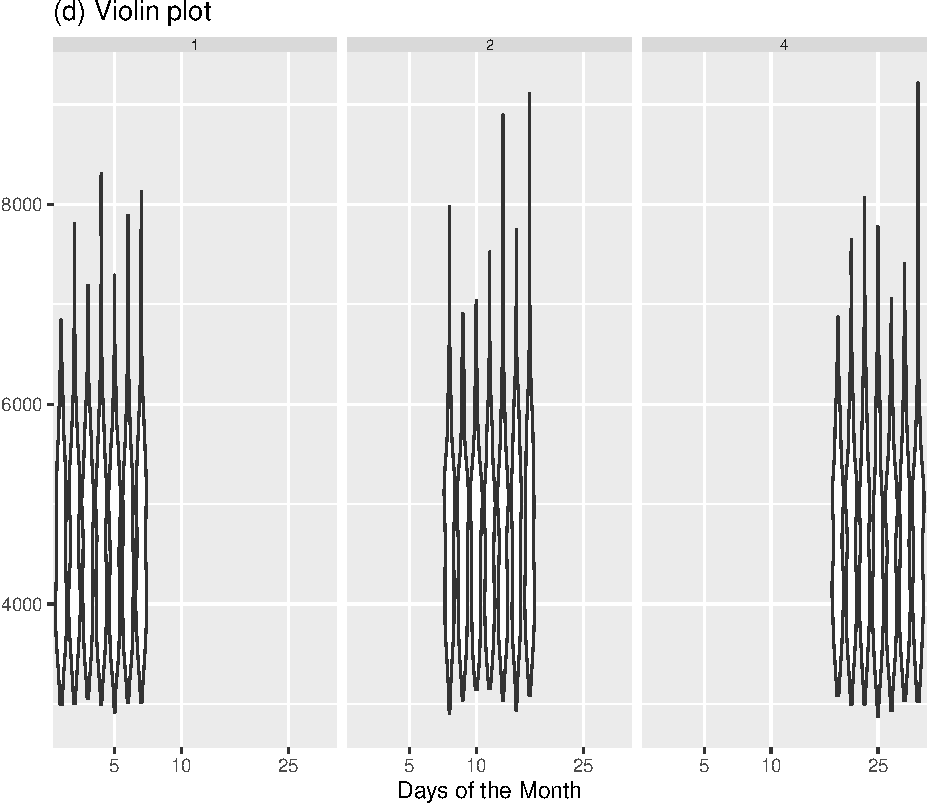
\includegraphics[width=0.5\linewidth]{figure/allFig-4} 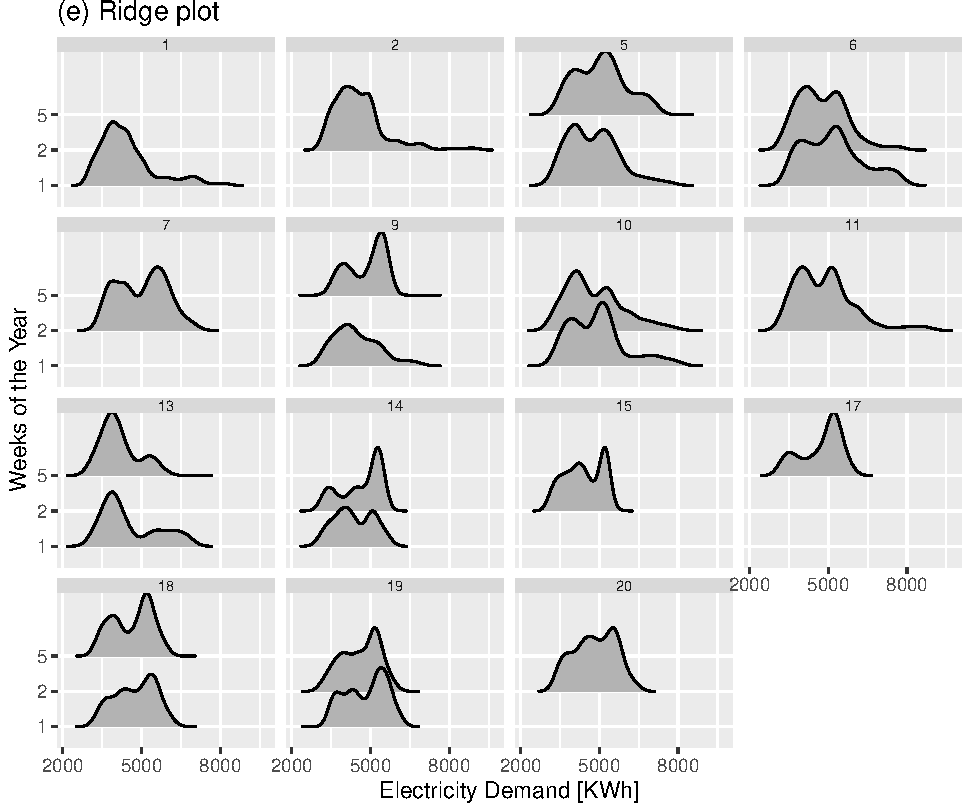
\includegraphics[width=0.5\linewidth]{figure/allFig-5} 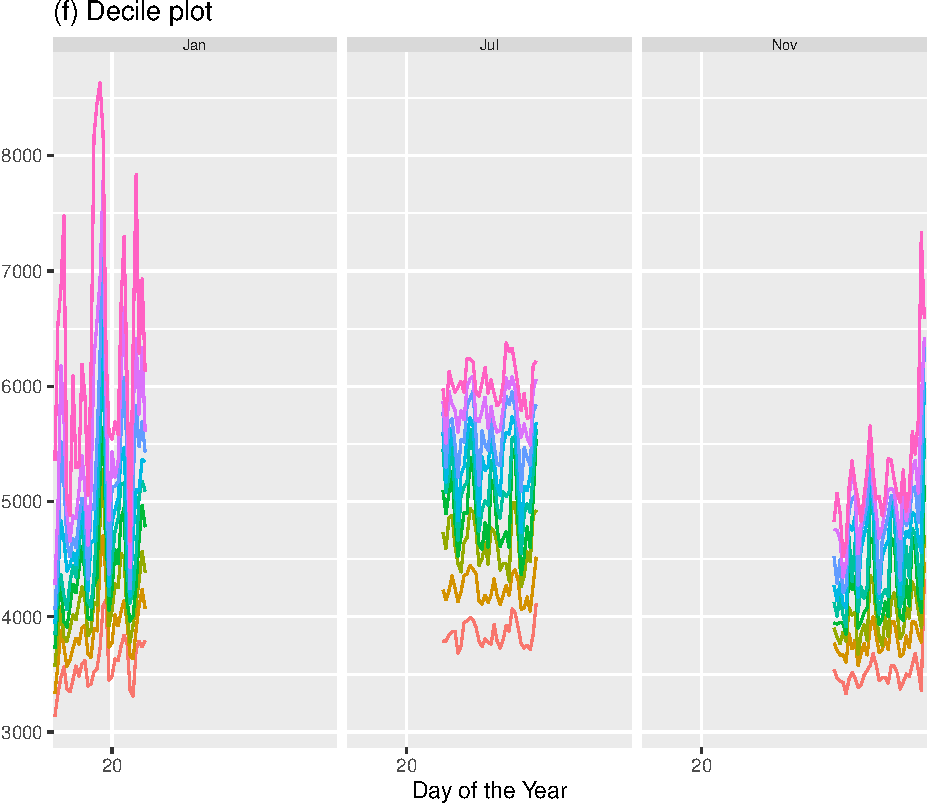
\includegraphics[width=0.5\linewidth]{figure/allFig-6} \hfill{}

\caption{Various probability distribution plots of electricity consumption data of Victoria from 2012 to 2014. (a) Letter value plot by DoM and MoY, (b) Decile plot by HoD and DoW (c) Box plot by DoY and DoM, (d) Violin plot of DoM and WoM, (e) Ridge plot by WoM and WoY, (f) Decile plot by DoY and MoY. Only plots (a) and (b) show harmonised time variables.}\label{fig:allFig}
\end{figure}

\hypertarget{effect-of-number-of-observations}{%
\subsection{Effect of number of
observations}\label{effect-of-number-of-observations}}

Even with harmonies, visualizing probability distributions can be
misleading either due to rarely occuring categories or unevenly
distributed events.

\hypertarget{rarely-occuring-events}{%
\subsubsection{Rarely occuring events}\label{rarely-occuring-events}}

Suppose we have \(T\) observations, and two cyclic granularities -
\(C_1\) with \(n\) categories and \(C_2\) with \(m\) categories. Each
element of \(C_1\) occurs approximately \(T/n\) times while each element
of \(C_2\) occurs approximately \(T/m\) times. There are no structurally
empty combinations, and each combination will occur on average an equal
number of times as \(T\rightarrow\infty\), so the average number of
observations per combination is \(T/(mn)\). If we require at least \(k\)
observations to create a meaningful panel, then provided \(T \ge mnk\),
the visualization will be acceptable. The value of \(k\) will depend on
what type of visualization we are producing. For a decile plot, even
\(k=10\) may be acceptable, but for density estimates, we would need
\(k \ge 30\). Rarely occurring categories such as the 366th day of the
year, or the 31st day of the month can suffer from such problem.

\hypertarget{unevenly-distributed-events}{%
\subsubsection{Unevenly distributed
events}\label{unevenly-distributed-events}}

Even when there are no rarely occuring events, number of observations
might vary hugely within or across each panel. This might happen due to
missing observations in the data or uneven locations of events in time
domain. In such cases, the visualizations that use kernel density
estimates should be used with caution as sample size would directly
affect both the variance of the estimator and the confidence intervals.
Measures such as Gini's coefficient may be used to see if sample sizes
vary widely across panels.

\hypertarget{sec:application}{%
\section{Applications}\label{sec:application}}

\hypertarget{sec:smartmeter}{%
\subsection{Smart meter data of Australia}\label{sec:smartmeter}}

Smart meters provide large quantities of measurements on energy usage
for households across Australia. One of the customer trial
\citep{smart-meter} conducted as part of the Smart Grid Smart City
(SGSC) project (2010-2014) in Newcastle, New South Wales and some parts
of Sydney provides customer wise data on half-hourly energy usage and
detailed information on appliance use, climate, retail and distributor
product offers, and other related factors. It would be interesting to
explore the energy consumption distribution for these customers and gain
more insights on their energy behavior which are otherwise lost either
due to aggregation or looking only at coarser temporal units. The idea
here is to show how looking at the time across different granularities
together can help identify different behavioral patterns and identify
the extreme and regular households amongst these 50 households.

In Figure \ref{fig:day-fortnight}, the smart meter data is filtered for
two customers to illustrate what kinds of insights can be drawn for the
energy behavior of these two customers. it can be seen that for most
days of the fortnight, the second household has much less consumption
than the first one. However, there is additional information that we can
derive looking at the distribution. If we consider letter value F as a
regular behavior and letter values beyond F as not-so-regular behavior,
we can conclude that the regular behavior of the first household is more
stable than the second household. However, the distribution of tail of
the first household is more variable, observed through distinct letter
values, implying that their not-so-regular behavior is quite extreme.
This shows, how looking at the distribution of the dependent variable
can throw more light on the energy behavior of the customers, which are
lost using aggregate or summary statistics.

\begin{figure}

{\centering 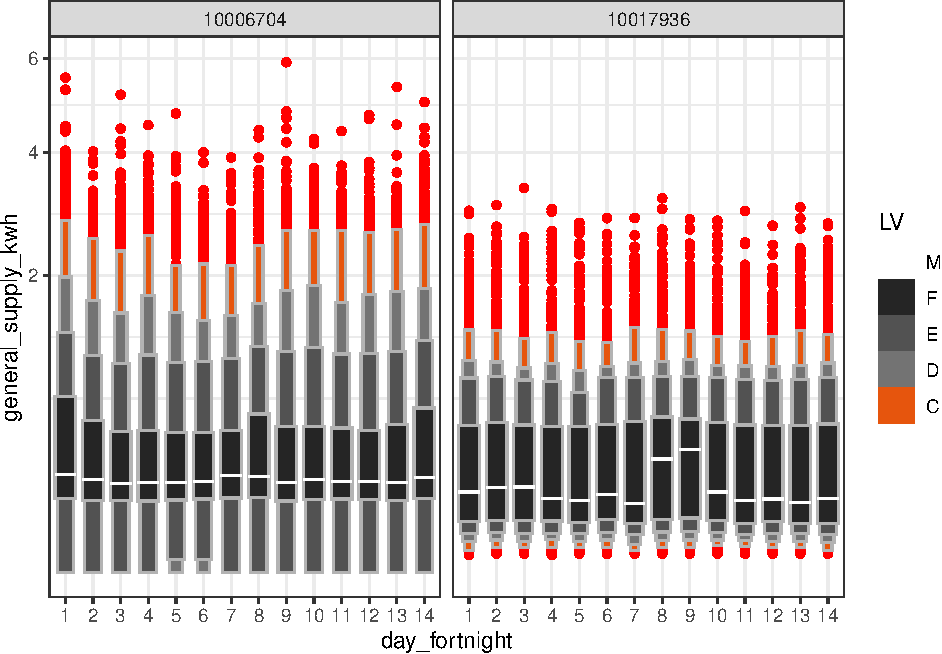
\includegraphics[width=\textwidth]{figure/day-fortnight-1} 

}

\caption{Letter value plot of two households across days of the fortnight. M, F, E, D and C represents the letter values of energy consumption. Regular behavior (within letter value F) is more variable for the 2nd household, whereas extreme behavior (beyond letter value F) is varying more for the first household.}\label{fig:day-fortnight}
\end{figure}

\textbf{gravitas} R package \citep{R-gravitas} is used to facilitate the
systematic exploration here. While trying to explore the energy behavior
of these customers systematically across cyclic time granularities, the
first thing we should have at our disposal is to know which all cyclic
time granularities we can look at exhaustively. If we consider
conventional time deconstructions for a Gregorian calendar (second,
minute, half-hour, hour, day, week, fortnight, month, quarter, semester,
year), the following time granularities can be considered for this
analysis.

\begin{verbatim}
#> 30m
\end{verbatim}

\begin{verbatim}
#>  [1] "hhour_hour"         "hhour_day"          "hhour_week"        
#>  [4] "hhour_fortnight"    "hhour_month"        "hhour_quarter"     
#>  [7] "hhour_semester"     "hhour_year"         "hour_day"          
#> [10] "hour_week"          "hour_fortnight"     "hour_month"        
#> [13] "hour_quarter"       "hour_semester"      "hour_year"         
#> [16] "day_week"           "day_fortnight"      "day_month"         
#> [19] "day_quarter"        "day_semester"       "day_year"          
#> [22] "week_fortnight"     "week_month"         "week_quarter"      
#> [25] "week_semester"      "week_year"          "fortnight_month"   
#> [28] "fortnight_quarter"  "fortnight_semester" "fortnight_year"    
#> [31] "month_quarter"      "month_semester"     "month_year"        
#> [34] "quarter_semester"   "quarter_year"       "semester_year"
\end{verbatim}

The interval of this tsibble is 30 minutes, and hence the temporal
granularities range from half-hour to year. If these options are
considered too many, the most coarse temporal unit can be set to be a
``month''.

\begin{verbatim}
#>  [1] "hhour_hour"      "hhour_day"       "hhour_week"     
#>  [4] "hhour_fortnight" "hhour_month"     "hour_day"       
#>  [7] "hour_week"       "hour_fortnight"  "hour_month"     
#> [10] "day_week"        "day_fortnight"   "day_month"      
#> [13] "week_fortnight"  "week_month"      "fortnight_month"
\end{verbatim}

Also, some intermediate temporal units that might not be pertinent to
the analysis can be removed from the list of cyclic granularities we
want to look at.

\begin{verbatim}
#> [1] "hour_day"   "hour_week"  "hour_month" "day_week"   "day_month" 
#> [6] "week_month"
\end{verbatim}

Now that we have the list of cyclic granularities to look at, we can
visualize the distribution. From the search list, we found six cyclic
granularities for which we would like to derive insights of energy
behavior. The distribution of energy needs to be visualized across two
cyclic granularities at a time. It is equivalent to taking 2
granularities from 6, which essentially is equivalent to visualizing 30
plots.However, harmony/clash pairs can identified among those 30 pairs,
to determine feasibility of plotting any pairs together. We are left
with 13 harmonies pair, each of which can be plotted together to look at
the energy behavior from different perspectives.

\begin{Shaded}
\begin{Highlighting}[]
\NormalTok{smart_meter10 }\OperatorTok\StringTok{ }\KeywordTok{harmony}\NormalTok{(}
  \DataTypeTok{ugran =} \StringTok{"month"}\NormalTok{,}
  \DataTypeTok{filter_out =} \KeywordTok{c}\NormalTok{(}\StringTok{"hhour"}\NormalTok{, }\StringTok{"fortnight"}\NormalTok{)}
\NormalTok{)}
\end{Highlighting}
\end{Shaded}

\begin{verbatim}
#> # A tibble: 13 x 4
#>    facet_variable x_variable facet_levels x_levels
#>    <chr>          <chr>             <int>    <int>
#>  1 day_week       hour_day              7       24
#>  2 day_month      hour_day             31       24
#>  3 week_month     hour_day              5       24
#>  4 day_month      hour_week            31      168
#>  5 week_month     hour_week             5      168
#>  6 day_week       hour_month            7      744
#>  7 hour_day       day_week             24        7
#>  8 day_month      day_week             31        7
#>  9 week_month     day_week              5        7
#> 10 hour_day       day_month            24       31
#> 11 day_week       day_month             7       31
#> 12 hour_day       week_month           24        5
#> 13 day_week       week_month            7        5
\end{verbatim}

\begin{Shaded}
\begin{Highlighting}[]
\NormalTok{smart_meter10 }\OperatorTok\StringTok{ }\KeywordTok{gran_advice}\NormalTok{(}\StringTok{"wknd_wday"}\NormalTok{, }\StringTok{"hour_day"}\NormalTok{)}
\end{Highlighting}
\end{Shaded}

\begin{verbatim}
#> The chosen granularities are harmonies 
#>  
#> Recommended plots are: violin lv quantile boxplot 
#>  
#> Number of observations are homogenous across facets 
#>  
#> Number of observations are homogenous within facets 
#>  
#> Cross tabulation of granularities : 
#>  
#> # A tibble: 24 x 3
#>    hour_day Weekday Weekend
#>    <fct>      <dbl>   <dbl>
#>  1 0           7705    3097
#>  2 1           7698    3100
#>  3 2           7698    3101
#>  4 3           7698    3102
#>  5 4           7699    3099
#>  6 5           7701    3098
#>  7 6           7700    3099
#>  8 7           7700    3098
#>  9 8           7695    3098
#> 10 9           7696    3098
#> # ... with 14 more rows
\end{verbatim}

In \autoref{fig:bothcust} we visualize the harmony pair (wknd\_wday,
hour\_day) through a box plot. Boxplot of energy consumption is shown
across wknd\_wday (facet) and hour-day (x-axis) for the same two
households. For the second household, outliers are less prominent
implying their regular behavior is more stable. For the first household,
energy behavior is not significantly different between weekdays and
weekends. For the second household, median energy consumption for the
early morning hours is extremely high for weekends compared to weekdays.

For the second household, outliers are less prominent implying their
regular behavior is more stable. For the first household, energy
behavior is not significantly different between weekdays and weekends.
For the second household, median energy consumption for the early
morning hours is extremely high for weekends compared to weekdays.

\begin{figure}

{\centering 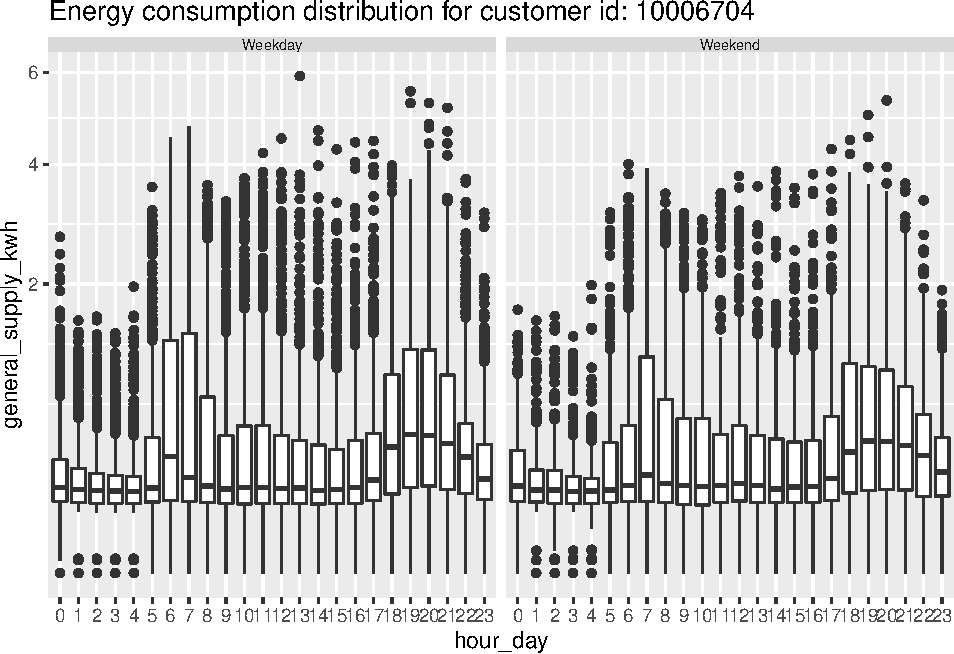
\includegraphics[width=\textwidth]{figure/bothcust-1} 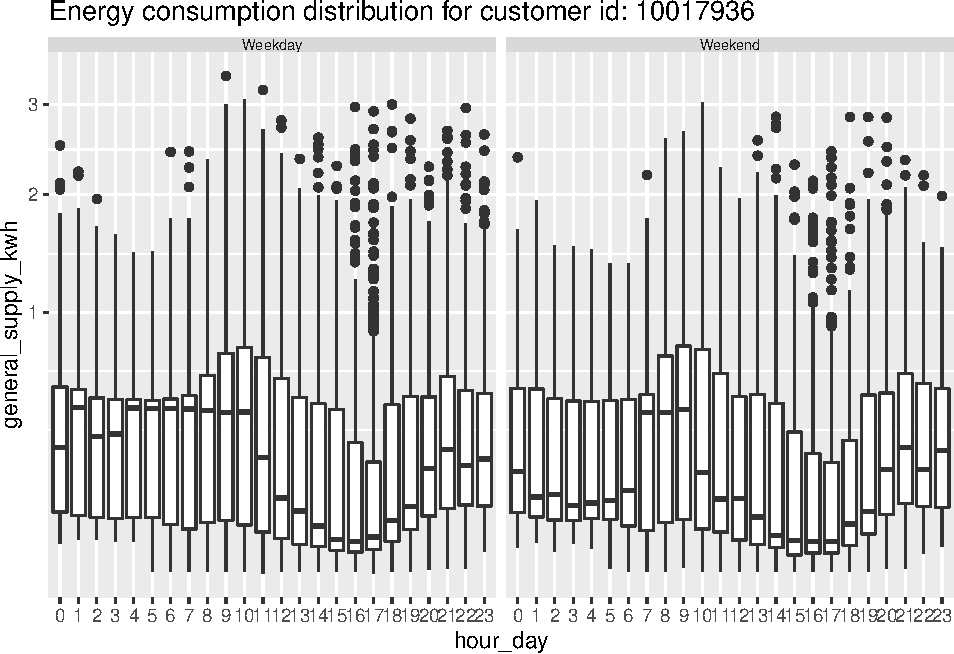
\includegraphics[width=\textwidth]{figure/bothcust-2} 

}

\caption{Boxplot of energy consumption across hours of the day faceted by weekday/weekend for household 1 (customer id: 10006704) and household 2 (customer id: 10017936). Median behavior for the early morning hours of household 2 is extremely high for weekends compared to weekdays, not much differenc can be observed for household 1. }\label{fig:bothcust}
\end{figure}

Now, we would like to see how these customers' behavior relate to the
rest of the 50 households across these two measures -

\begin{itemize}
\item
  if energy distribution is skewed towards extreme?
\item
  if the weekend and weekday behavior are different for most of these
  households?
\end{itemize}

Figure \ref{fig:wknd-wday50} shows the quantile plot of energy
consumption of 50 households. Similar quantiles for weekend and weekdays
indicate that behaviors of most of these customers do not alter between
weekdays and weekends.

Figure \ref{fig:my-hd} shows that the median is very close to the lower
boundaries of all the other bands implying energy consumption for these
households are left skewed. Moreover, only the pink band changes
significantly in winter months (May - August). The median consumption or
width of other bands doesn't vary much across seasons, implying extreme
behavior or extreme customers does not vary across seasons much. Most of
the behavioral changes occur in the quartiles, that too in peak hours of
the day. It is to be noted here that the the level of quantiles
increased too in winter months (obvious because of weather conditions),
the interesting part is to notice that the relationship between bands
other than quartile stayed same across seasons.

\begin{figure}

{\centering 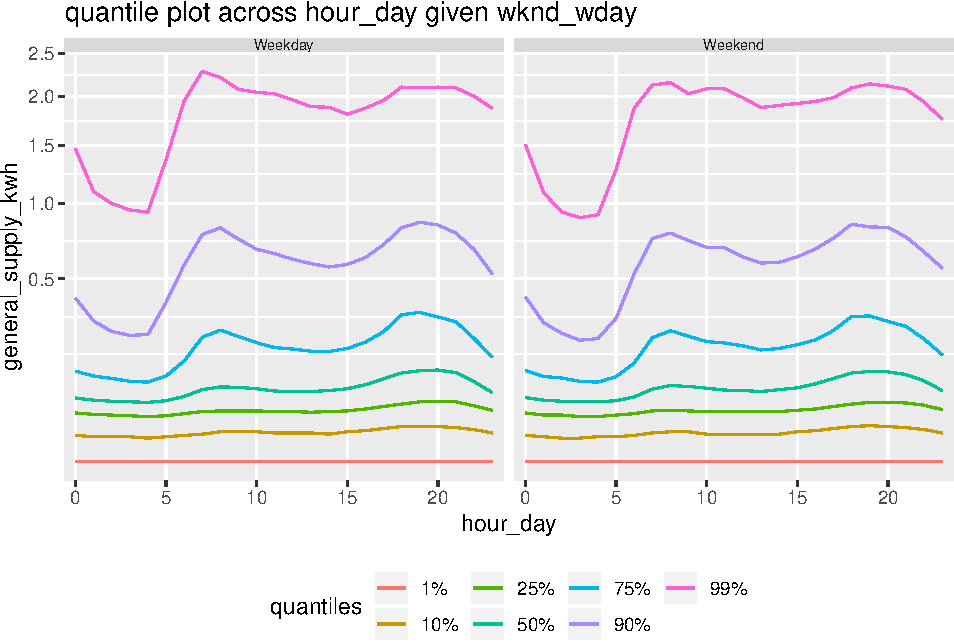
\includegraphics[width=\textwidth]{figure/wknd-wday50-1} 

}

\caption{Quantile plot of energy consumption of 50 households across different hours of the day faceted by weekday and weekend. The quantiles are not different for weekdays and weekends implying either the behavior balances out among these customers or most of them do not behave differently for weekdays and weekends.}\label{fig:wknd-wday50}
\end{figure}

\begin{figure}

{\centering 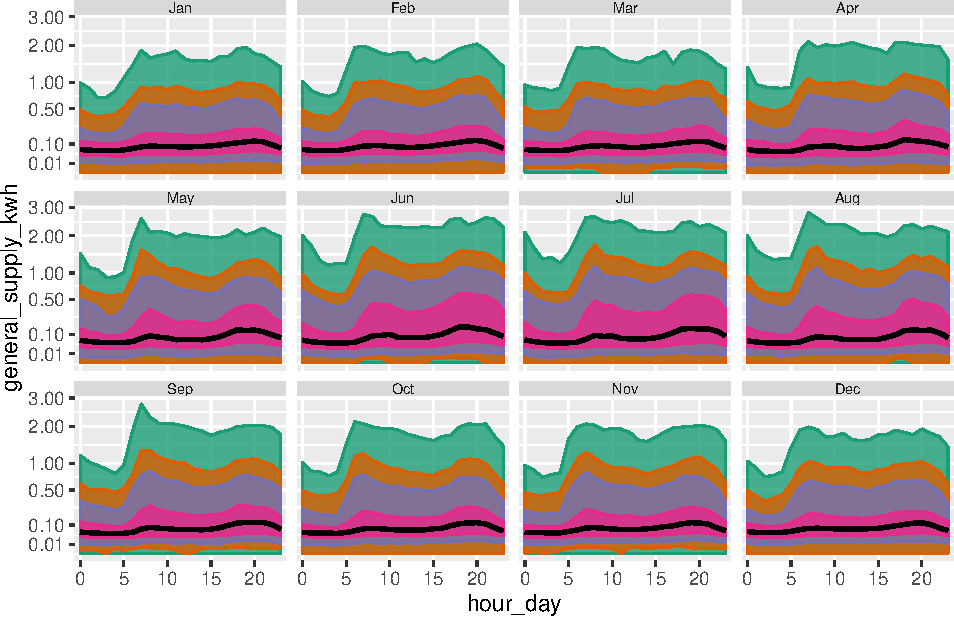
\includegraphics[width=\textwidth]{figure/my-hd-1} 

}

\caption{Area quantile plots of energy consumption across hours of the day faceted by months of the year. The black line is the median, whereas the pink band covers 25th to 75th percentile, the orange band covers 10th to 90th percentile and the green band covers 1st to 99th percentile. The median and quartile consumption increase in winter months, but extreme behavior represented by higher bands mostly stay the same across seasons. }\label{fig:my-hd}
\end{figure}

This case study shows systematic exploration of energy behavior starting
with two households and comparing some of their features with all 50
households. First, it helps us to find the list of granularities to look
at, then shrinks the number of possible visualizations by identifying
harmonies and then explored harmony pairs to gain some insights on
periodic behavior of the households.

\hypertarget{sec:cricket}{%
\subsection{T20 cricket data of Indian Premiere
League}\label{sec:cricket}}

The application is not only restricted to temporal data. We provide an
example of cricket to illustrate how this can be generalized in other
applications. The Indian Premier League (IPL) is a professional Twenty20
cricket league in India contested by eight teams representing eight
different cities in India. With eight teams, each team plays each other
twice in a home-and-away round-robin format in the league phase. In a
Twenty20 game the two teams have a single innings each, which is
restricted to a maximum of 20 overs. Hence, in this format of cricket, a
match will consist of 2 innings, an innings will consist of 20 overs, an
over will consist of 6 balls with some exceptions.

The ball by ball data for IPL season 2008 to 2016 is fetched from
\href{https://www.kaggle.com/josephgpinto/ipl-data-analysis/data}{Kaggle}.
The \texttt{cricket} data set in the \texttt{gravitas} package
summarizes the ball-by-ball data cross overs and contains information
for a sample of 214 matches spanning 9 seasons (2008 to 2016).

Although there is no conventional time granularity in cricket, we can
still represent the data set \texttt{cricket} through a
\texttt{tsibble}, where each over, which represents an ordering from
past to future, can form the index of the tsibble. The hierarchy table
would look like the following:

\begin{longtable}[]{@{}lr@{}}
\toprule
G & k\tabularnewline
\midrule
\endhead
over & 20\tabularnewline
inning & 2\tabularnewline
match & 1\tabularnewline
\bottomrule
\end{longtable}

There are many interesting questions that can possibly be answered with
such a data set, however, we will explore a few and understand how the
proposed approach in the paper can help answer some of the questions.

First, we look at the distribution of runs per over across over of the
innings and seasons in \autoref{fig:seas-over-inning}. The distribution
of runs per over has not significantly changed from 2008 to 2016. There
is no clear pattern/trend that runs per over is increasing or decreasing
across seasons. Hence, we work with subsets of seasons to answer some of
the questions:

Q1: How run rates vary depending on if a team bats first or second?

Mumbai Indians(MI) and Chennai Super kings(CSK) are considered one of
the best teams in IPL with multiple winning titles and always appearing
in final 4 from 2010 to 2015. It would be interesting to take their
example in order to dive deeper into the first question.

\begin{figure}

{\centering 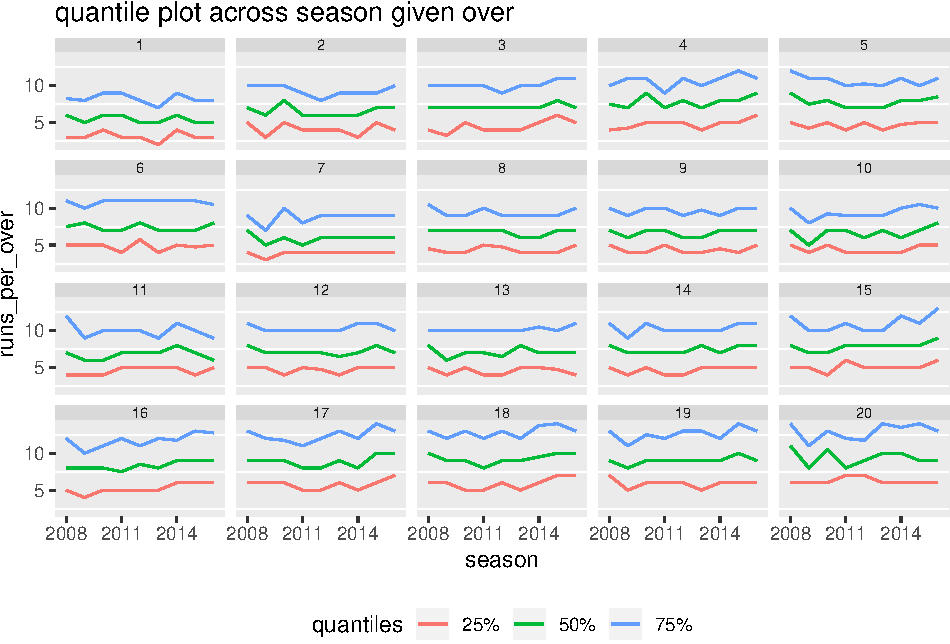
\includegraphics[width=\textwidth]{figure/seas-over-inning-1} 

}

\caption{Quantile plot of runs per over across overs of different seasons. There is no pattern on increase or decrease of runs across overs for seasons.}\label{fig:seas-over-inning}
\end{figure}

From Figure \ref{fig:cricex}, it can be observed that there is no clear
upward shift in runs in the second innings as compared to the first
innings. The variability of runs also increases as the teams approach
towards the end of the innings, as observed through the longer and more
distinct letter values.

\begin{figure}

{\centering 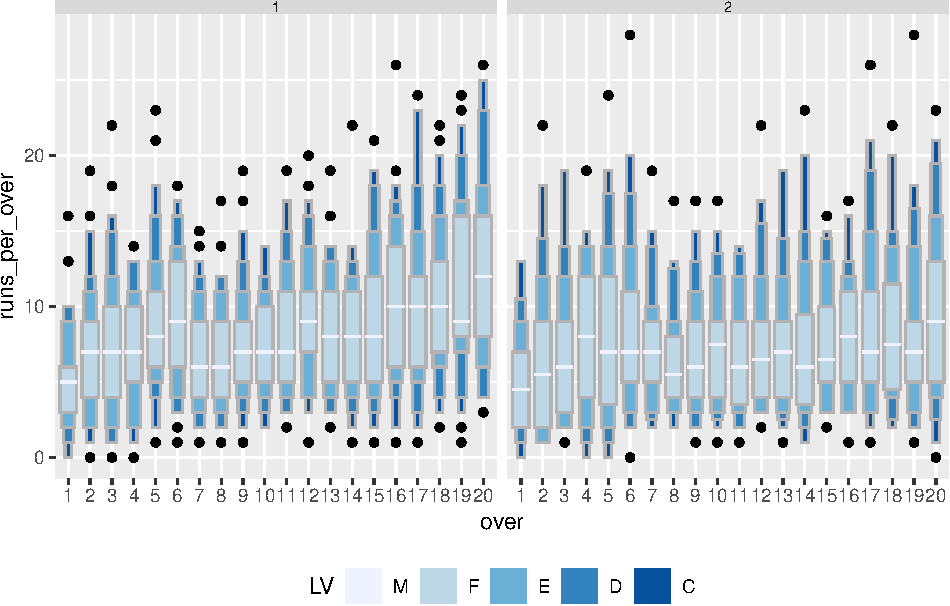
\includegraphics[width=\textwidth]{figure/cricex-1} 

}

\caption{Letter value plot of runs per over across overs of the inning faceted by innings of the match. No upward shift in runs in the second innings like that in the first implying teams are more vulnerable to score more in the first innings as they approach the end of the inning.}\label{fig:cricex}
\end{figure}

Q2: Is run rate set to reduce in subsequent over if fielding/bowling is
good in the previous over? Between fielding and bowling which penalizes
runs in the subsequent over more?

For establishing that the fielder fielded well in a particular over, we
can see how many catches and run outs were made in that particular over.
If a batsman is bowled out, it does not necessarily signify good
fielding. So we only include catches and run out as a measure of
fielding. Difference in runs across over should be negative if good
fielding has an impact on the runs scored in the subsequent overs. Let
us see if this fact is true. Figure \ref{fig:field} shows the difference
between run rate between two subsequent overs are negative when good
fielding leads to one or two dismissals in an over, implying good
fielding in one over has indeed an impact on runs scored in the
subsequent overs.

\begin{verbatim}
#> # A tibble: 4 x 21
#>   fielding_wckts   `1`   `2`   `3`   `4`   `5`   `6`   `7`   `8`   `9`
#>   <fct>          <dbl> <dbl> <dbl> <dbl> <dbl> <dbl> <dbl> <dbl> <dbl>
#> 1 0               1039   997   972   978   962   957  1002  1012   993
#> 2 1                120   145   171   165   180   181   138   124   140
#> 3 2                  5    10     8     8     9    10     6    10     8
#> 4 3                  0     0     0     0     0     0     0     0     0
#> # ... with 11 more variables: `10` <dbl>, `11` <dbl>, `12` <dbl>,
#> #   `13` <dbl>, `14` <dbl>, `15` <dbl>, `16` <dbl>, `17` <dbl>,
#> #   `18` <dbl>, `19` <dbl>, `20` <dbl>
\end{verbatim}

\begin{figure}

{\centering 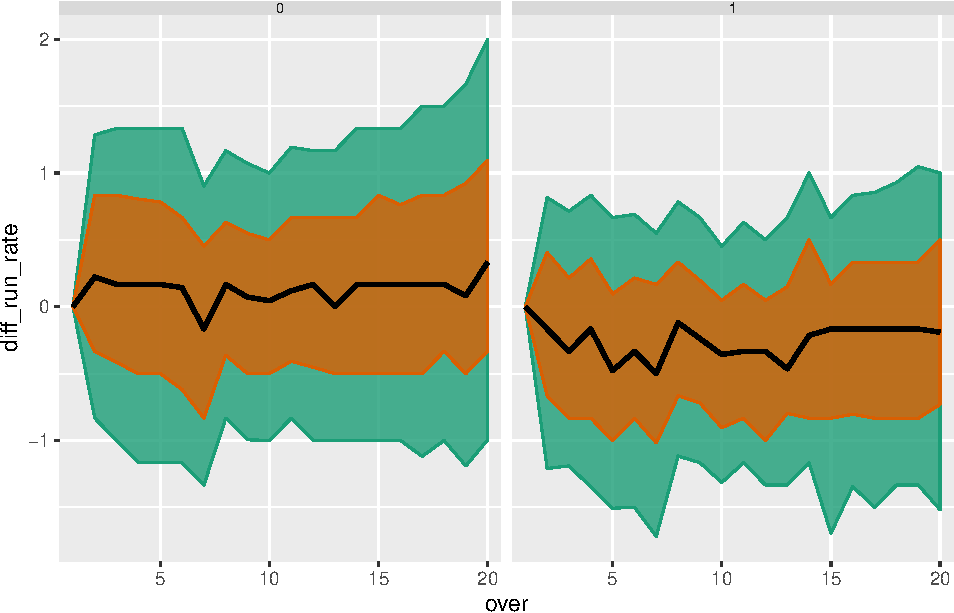
\includegraphics[width=\textwidth]{figure/field-1} 

}

\caption{Distribution of lagged run rate across overs of the innings and dismissals by catch and catch and bowled. This shows good fielding in one over leads to lower runs in the subsequent overs for at least 50 percentiles of times.}\label{fig:field}
\end{figure}

Q3: Is runs set to reduce in the next over for dot balls in this over?

A dot ball is a delivery bowled without any runs scored off it. The
number of dot balls is reflective of the quality of bowling in the game.
Run rate of an over should ideally decrease if the number of dot balls
increase. However, what is the effect of dot balls on runs scored in the
subsequent over. Will players batsman likely to go for big shots because
they couldn't score good runs in the previous over? Or they should play
consistently and avoid scoring high? From figure \ref{fig:exdot} shows
the quantile plot of runs across overs for none, one or two dot balls
per over in the facets. Each of the quantiles decrease across facets.
With two dot balls per over, at least 50\% of the times, run rates
decrease in the subsequent over as observed through the negative values
for 10th, 25th and 50th percentile quantiles.

\begin{figure}[htb]

{\centering 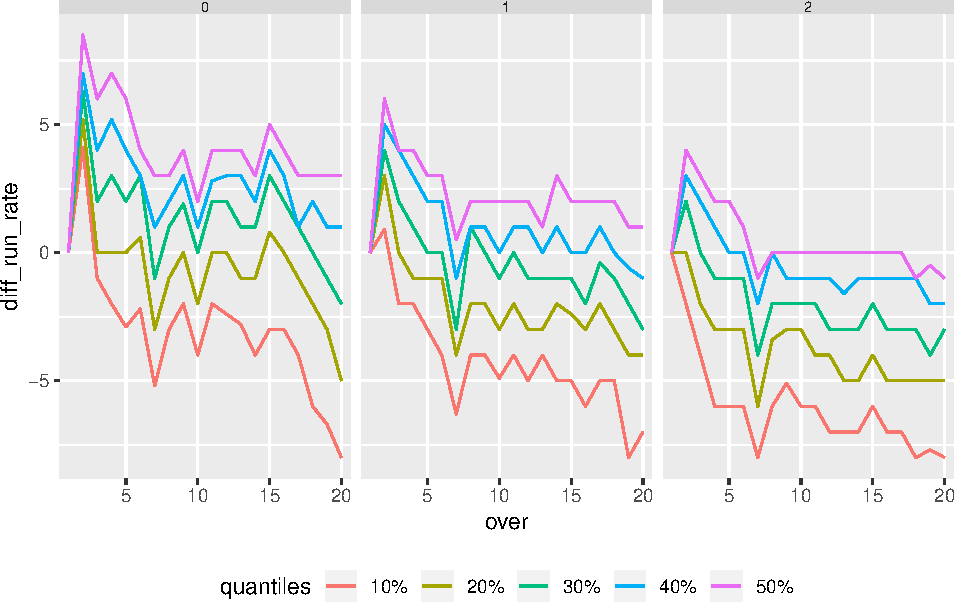
\includegraphics[width=\textwidth]{figure/exdot-1} 

}

\caption{10th, 20th, 30th, 40th and 50th quantiles of runs per over are drawn  across overs of the innings with no (facet 1), one (facet 2) and two (facet 3) dot balls per over. For all three cases, difference in runs between subsequent overs decrease.}\label{fig:exdot}
\end{figure}

\hypertarget{sec:discussion}{%
\section{Discussion}\label{sec:discussion}}

\hypertarget{acknowledgements}{%
\section*{Acknowledgements}\label{acknowledgements}}
\addcontentsline{toc}{section}{Acknowledgements}

\hypertarget{bibliography}{%
\section{Bibliography}\label{bibliography}}

--\textgreater{}

\bibliographystyle{agsm}
\bibliography{bibliography.bib}

\end{document}
